% Options for packages loaded elsewhere
\PassOptionsToPackage{unicode}{hyperref}
\PassOptionsToPackage{hyphens}{url}
\PassOptionsToPackage{dvipsnames,svgnames,x11names}{xcolor}
%
\documentclass[
  letterpaper,
  DIV=11,
  numbers=noendperiod]{scrartcl}

\usepackage{amsmath,amssymb}
\usepackage{iftex}
\ifPDFTeX
  \usepackage[T1]{fontenc}
  \usepackage[utf8]{inputenc}
  \usepackage{textcomp} % provide euro and other symbols
\else % if luatex or xetex
  \usepackage{unicode-math}
  \defaultfontfeatures{Scale=MatchLowercase}
  \defaultfontfeatures[\rmfamily]{Ligatures=TeX,Scale=1}
\fi
\usepackage{lmodern}
\ifPDFTeX\else  
    % xetex/luatex font selection
\fi
% Use upquote if available, for straight quotes in verbatim environments
\IfFileExists{upquote.sty}{\usepackage{upquote}}{}
\IfFileExists{microtype.sty}{% use microtype if available
  \usepackage[]{microtype}
  \UseMicrotypeSet[protrusion]{basicmath} % disable protrusion for tt fonts
}{}
\makeatletter
\@ifundefined{KOMAClassName}{% if non-KOMA class
  \IfFileExists{parskip.sty}{%
    \usepackage{parskip}
  }{% else
    \setlength{\parindent}{0pt}
    \setlength{\parskip}{6pt plus 2pt minus 1pt}}
}{% if KOMA class
  \KOMAoptions{parskip=half}}
\makeatother
\usepackage{xcolor}
\setlength{\emergencystretch}{3em} % prevent overfull lines
\setcounter{secnumdepth}{2}
% Make \paragraph and \subparagraph free-standing
\ifx\paragraph\undefined\else
  \let\oldparagraph\paragraph
  \renewcommand{\paragraph}[1]{\oldparagraph{#1}\mbox{}}
\fi
\ifx\subparagraph\undefined\else
  \let\oldsubparagraph\subparagraph
  \renewcommand{\subparagraph}[1]{\oldsubparagraph{#1}\mbox{}}
\fi


\providecommand{\tightlist}{%
  \setlength{\itemsep}{0pt}\setlength{\parskip}{0pt}}\usepackage{longtable,booktabs,array}
\usepackage{calc} % for calculating minipage widths
% Correct order of tables after \paragraph or \subparagraph
\usepackage{etoolbox}
\makeatletter
\patchcmd\longtable{\par}{\if@noskipsec\mbox{}\fi\par}{}{}
\makeatother
% Allow footnotes in longtable head/foot
\IfFileExists{footnotehyper.sty}{\usepackage{footnotehyper}}{\usepackage{footnote}}
\makesavenoteenv{longtable}
\usepackage{graphicx}
\makeatletter
\def\maxwidth{\ifdim\Gin@nat@width>\linewidth\linewidth\else\Gin@nat@width\fi}
\def\maxheight{\ifdim\Gin@nat@height>\textheight\textheight\else\Gin@nat@height\fi}
\makeatother
% Scale images if necessary, so that they will not overflow the page
% margins by default, and it is still possible to overwrite the defaults
% using explicit options in \includegraphics[width, height, ...]{}
\setkeys{Gin}{width=\maxwidth,height=\maxheight,keepaspectratio}
% Set default figure placement to htbp
\makeatletter
\def\fps@figure{htbp}
\makeatother
% definitions for citeproc citations
\NewDocumentCommand\citeproctext{}{}
\NewDocumentCommand\citeproc{mm}{%
  \begingroup\def\citeproctext{#2}\cite{#1}\endgroup}
\makeatletter
 % allow citations to break across lines
 \let\@cite@ofmt\@firstofone
 % avoid brackets around text for \cite:
 \def\@biblabel#1{}
 \def\@cite#1#2{{#1\if@tempswa , #2\fi}}
\makeatother
\newlength{\cslhangindent}
\setlength{\cslhangindent}{1.5em}
\newlength{\csllabelwidth}
\setlength{\csllabelwidth}{3em}
\newenvironment{CSLReferences}[2] % #1 hanging-indent, #2 entry-spacing
 {\begin{list}{}{%
  \setlength{\itemindent}{0pt}
  \setlength{\leftmargin}{0pt}
  \setlength{\parsep}{0pt}
  % turn on hanging indent if param 1 is 1
  \ifodd #1
   \setlength{\leftmargin}{\cslhangindent}
   \setlength{\itemindent}{-1\cslhangindent}
  \fi
  % set entry spacing
  \setlength{\itemsep}{#2\baselineskip}}}
 {\end{list}}
\usepackage{calc}
\newcommand{\CSLBlock}[1]{\hfill\break\parbox[t]{\linewidth}{\strut\ignorespaces#1\strut}}
\newcommand{\CSLLeftMargin}[1]{\parbox[t]{\csllabelwidth}{\strut#1\strut}}
\newcommand{\CSLRightInline}[1]{\parbox[t]{\linewidth - \csllabelwidth}{\strut#1\strut}}
\newcommand{\CSLIndent}[1]{\hspace{\cslhangindent}#1}

% load packages
\usepackage{geometry}
\usepackage{eso-pic}

%% Set page size with a wider right margin
\geometry{a4paper, left=25mm, top=25mm, bottom=25mm, right=25mm}

%% Let's add a logo to the bottom right
\AddToShipoutPicture{% 
     % logo
    \AtPageLowerLeft{% start the bar at the bottom right of the page
        \put(\LenToUnit{\dimexpr\paperwidth-195mm},1cm){% move it to the top right
            \color{white}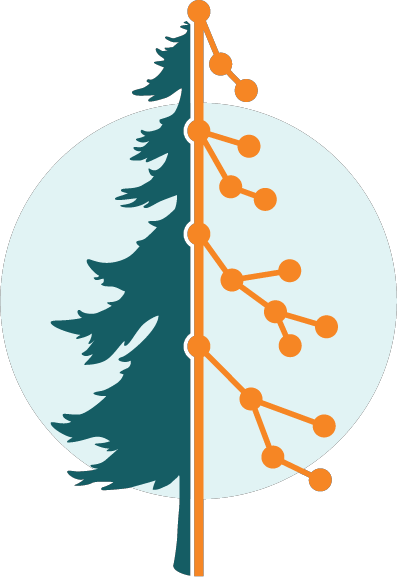
\includegraphics[width=1cm]{assets/nwpage_tree_logo.png}
          }%
     }%
}
\KOMAoption{captions}{tableheading}
\makeatletter
\@ifpackageloaded{caption}{}{\usepackage{caption}}
\AtBeginDocument{%
\ifdefined\contentsname
  \renewcommand*\contentsname{Table of contents}
\else
  \newcommand\contentsname{Table of contents}
\fi
\ifdefined\listfigurename
  \renewcommand*\listfigurename{List of Figures}
\else
  \newcommand\listfigurename{List of Figures}
\fi
\ifdefined\listtablename
  \renewcommand*\listtablename{List of Tables}
\else
  \newcommand\listtablename{List of Tables}
\fi
\ifdefined\figurename
  \renewcommand*\figurename{Figure}
\else
  \newcommand\figurename{Figure}
\fi
\ifdefined\tablename
  \renewcommand*\tablename{Table}
\else
  \newcommand\tablename{Table}
\fi
}
\@ifpackageloaded{float}{}{\usepackage{float}}
\floatstyle{ruled}
\@ifundefined{c@chapter}{\newfloat{codelisting}{h}{lop}}{\newfloat{codelisting}{h}{lop}[chapter]}
\floatname{codelisting}{Listing}
\newcommand*\listoflistings{\listof{codelisting}{List of Listings}}
\makeatother
\makeatletter
\makeatother
\makeatletter
\@ifpackageloaded{caption}{}{\usepackage{caption}}
\@ifpackageloaded{subcaption}{}{\usepackage{subcaption}}
\makeatother
\ifLuaTeX
  \usepackage{selnolig}  % disable illegal ligatures
\fi
\usepackage{bookmark}

\IfFileExists{xurl.sty}{\usepackage{xurl}}{} % add URL line breaks if available
\urlstyle{same} % disable monospaced font for URLs
\hypersetup{
  pdftitle={Data Integration and Quality Assurance of Sequencing Metadata in Washington State},
  pdfkeywords={Sequencing, COVID19},
  colorlinks=true,
  linkcolor={blue},
  filecolor={Maroon},
  citecolor={Blue},
  urlcolor={Blue},
  pdfcreator={LaTeX via pandoc}}

\title{Data Integration and Quality Assurance of Sequencing Metadata in
Washington State}
\author{Frank Aragona \and Cory Yun \and Philip Crain \and Paul
Lloyd \and Emily Nebergall \and Cameron Ashton \and Peter J
Gibson \and Marcela Torres \and Lauren Frisbie \and Allison
Warren \and Laura Beilsmith \and Xichi Zhang \and Allison
Thibodeau \and Sarah Menz \and Topias Lemetyinen \and Alli
Black \and Alex Cox}
\date{2024-03-04}

\begin{document}
\maketitle
\begin{abstract}
Genomic surveillance is important for identifying and tracking SARS
CoV-2 variants to better mitigate spread of COVID-19. Washington State
Department of Health quickly increased capacity to surveil SARS CoV-2
variants by partnering with over 25 labs to collect sequencing data
while developing and implementing solutions to standardize submissions
and enhance data linkage and quality. High impact solutions included
development of a standardized reporting template, collection of case
demographics, adaptation of HL7 messages with sequencing data, and
strategic utilization of external sequencing data repositories. We
developed an automated pipeline that combines data science tools to
ingest, clean, and link SARS CoV-2 sequencing data from multiple
sources, while accounting for differing data formats and quality. This
manuscript details the first version of the pipeline developed in
February 2021 when processes were unstable and were being developed as
they were utilized.
\end{abstract}

\renewcommand*\contentsname{Table of contents}
{
\hypersetup{linkcolor=}
\setcounter{tocdepth}{3}
\tableofcontents
}
\section{Introduction}\label{introduction}

This manuscript documents the original data integration pipeline for
SARS-CoV-2 sequences for Washington State Department of Health during
early 2021 to mid 2023. The Sequencing project began in February 2021 as
an effort to process sequencing data into the Washington State Disease
Reporting System (WDRS). In turn, the data fuels SARS-CoV-2 variant
tracking and the generation of Covid-19 reports which are disseminated
to the highest levels of state government. The pipeline continuously
links data to our main database WDRS, where the data can be used to gain
insights via surveillance reports or research (for example, see Oltean
et al. n.d.; Oltean et al. 2024; Wagner et al. 2023). Data are processed
via numerous R/Python/SQL scripts and are uploaded via rosters (.csv
files) into WDRS and our Molecular Epidemiology produces
\href{https://doh.wa.gov/sites/default/files/2022-02/420-316-SequencingAndVariantsReport.pdf}{reports}
with the data. These processes ebb and flow often as changes are needed
regularly in response to the data that are received. Since mid 2023 we
have stopped using this particular pipeline and have built a new
pipeline using a more streamlined approach. The purpose of detailing the
original pipeline in this document is to give a transparent look at how
data were processed under the unusual circumstances during the COVID-19
pandemic. Many aspects of this pipeline are inefficient because it was
built under a rapidly changing environment, one that had never been
built before, in addition to the many time constraints placed on our
teams to produce data reports quickly. Some of the inefficiencies
exposed in this pipeline still exist with our newer pipelines, but our
teams are working to build a more sustainable way to process sequencing
data of any disease type.

There are a multitude of barriers which make data processing difficult
with any pipeline such as:

\begin{enumerate}
\def\labelenumi{\arabic{enumi}.}
\tightlist
\item
  Data standardization; data are received multiple ways. Depending on
  the manner it is submitted it may not follow the standard format
  requested from submitters. This requires manual intervention or
  communication back to labs. In addition, some submitters cannot change
  the manner in which they submit data which makes standardization
  across all labs impossible. These are handled by separate processes.
  Occasionally, submitters may break consistency in their own manner of
  which they report as well.
\item
  Data quality; the quality of data received from labs can vary
  dramatically. Data needs to match between three sources: Lab
  Submissions, WDRS, and GISAID. When the wrong data are sent this can
  make matching impossible and prevents records from making it into our
  systems. It has been found that submitters sometimes submit incorrect
  ACCESSION ID's that are used to match records between systems. Without
  the correct data it requires a considerable amount of manual
  intervention to be able to roster those records. Additionally, there
  are considerable lag times between all three data points/repositories;
  when a record is submitted that are not within WDRS the records cannot
  be matched and rostered.
\item
  Technological gaps; the COVID-19 pandemic has exposed many
  technological gaps in our public health disease surveillance systems.
  Much of the technology used for processing and storing data needed to
  be built out during early 2020 so that we could provide disease
  reports in a timely manner. Therefore a lot of processes like this
  pipeline were built for short term needs, adding on more and more
  `technological debt'. Short term solutions have consequences and our
  data infrastructure is not well suited for pipelines like this.
\end{enumerate}

The original pipeline aggregates sequencing data submitted via secure
file transfer, electronic lab reporting, lab management software, and
open access data repositories. The process incorporates robust solutions
to data challenges, including lagged data availability, variable data
formatting, record duplication, and missing data. After aggregation, the
pipeline connects records to COVID-19 case data via sequence to
diagnostic test identifiers. We used patient demographics and string
matching to link sequences to cases that are missing the unique
identifiers. Internal databases are compared to external repositories to
identify new results, track missing data, onboard new sequencing
partners, and validate data. This pipeline was able to mostly automate
aggregation, cleaning, and linkage of SARS CoV-2 genomic surveillance
data, minimizing manual work and hastening availability of data for
analysis and reporting.

Challenges remain despite these improvements in data standardization and
management. Barriers include differences in HL7 message reporting
capabilities among submitters, inconsistencies in virus naming
conventions, challenges in pulling data from public repositories, and
limitations within our current internal database infrastructure. These
factors increase likelihood of errors, require data processing logic
unique to individual submitters and require manual intervention.
Continued development of national standards can address these issues.
Data accessibility can be improved by encouraging open-source sharing,
especially to repositories that enable full programmatic data sourcing
for all users. A community of practice across departments of health to
discuss storage methods, processing pipelines, and matching approaches
would enhance current practices, and support greater consistency and
interoperability across public health.

\subsection{Timeline}\label{timeline}

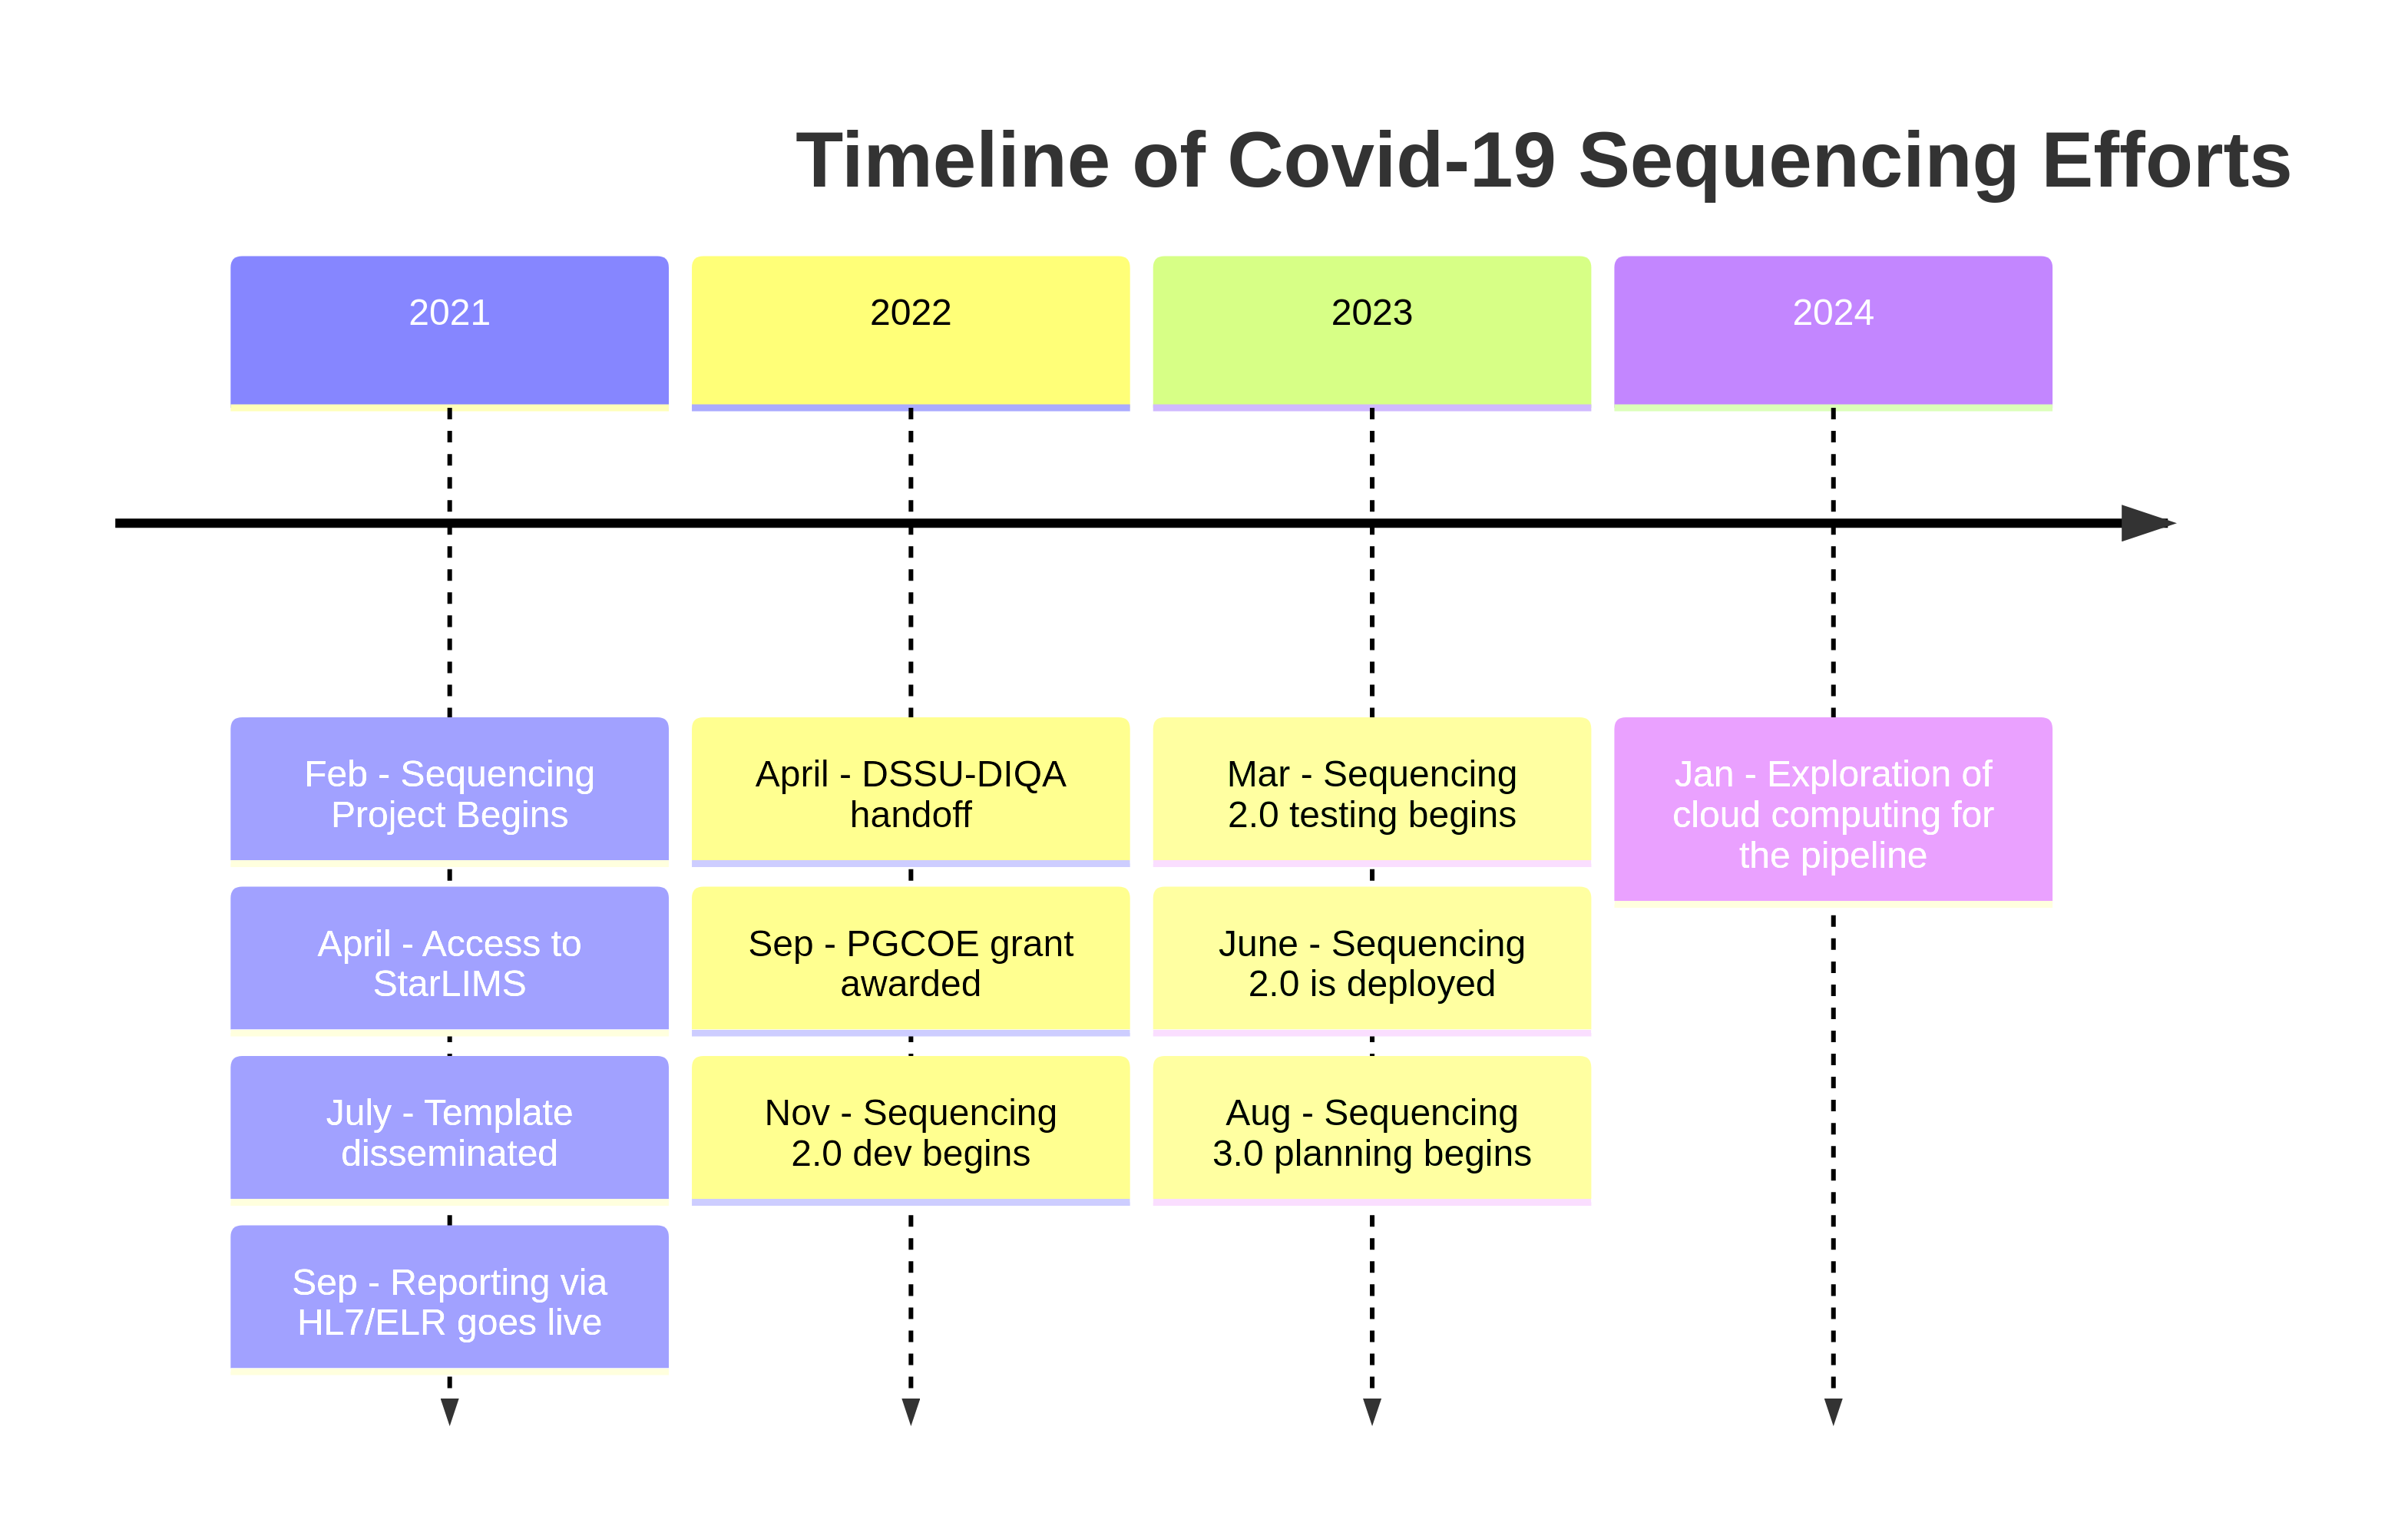
\includegraphics[width=7in,height=4.47in]{index_files/figure-latex/mermaid-figure-13.png}

\textsubscript{Source:
\href{https://NW-PaGe.github.io/sequencing_integration_pipeline1.0/index.qmd.html}{Article
Notebook}}

The sequencing metadata linkage project began in February 2021 by the
Data Science Support Unit (DSSU). A pipeline was needed to process and
upload sequencing data to Washington Disease Reporting System (WDRS) for
variant tracking/generation of reports to the governor's
office\hspace{0pt}. The pipeline links sequencing metadata to case data
in WDRS, links sequences to GISAID (Global Initiative on Sharing All
Influenza Data, a public sequencing repository), and it cleans and
transforms non-standardized data.

The project originally started as a group of individual contributors
writing R scripts to handle needs for pulling data and cleaning,
matching, and transforming non-standardized sequencing data\hspace{0pt}.
During this period, urgency was prioritized at the cost of technical
debt: it was a ``build as we go''\hspace{0pt} mentality given the time
restraints during the pandemic. This scenario made for segmented
processes and no true workflow. During height of the 2021-2022 period
this pipeline would typically process 1000+ records per
week\hspace{0pt}.

\section{General Overview}\label{sec-overview}

Sequencing data gets sent through our pipeline through multiple
processes and the pipeline works in the following steps:

\begin{enumerate}
\def\labelenumi{\arabic{enumi}.}
\tightlist
\item
  A submitter sends us the sequencing data three different ways;

  \begin{itemize}
  \tightlist
  \item
    as tabular data via secure file transfer (SFT)
  \item
    as tabular data that is `scraped' web-scraping of their dashboard as
    is the case with our PHL
  \item
    via ELR or electronic lab reporting that is automatically connected
    to our database
  \end{itemize}
\item
  Our pipeline will extract, transform, and link that data to a case in
  WDRS
\item
  The pipeline then performs quality checks to make sure errors or data
  leaks did not occur
\end{enumerate}

The three main routes that a submitter can send us data through are
detailed in Figure~\ref{fig-overview} under Template Submitters (secure
file transfer of tabular data), PHL (webscraping of tabular data), and
HL7 messages (secure data transfer for ELR).

First, the \href{@sec-template}{Template Submitters} script processes
the majority of data received by external submitters. Sequencing data
from external submitters are received via \texttt{.csv} files in a
template format which they uploaded to our secure file transfer (SFT)
portal.

Second, the The \href{@sec-phl}{PHL Roster} script processes the data
received from PHL (Public Health Laboratory), our internal laboratory.
Sequencing data from PHL is pulled from an internal dashboard,
`StarLIMS'. The logic for both processes are similar. There is an
attempt to link the sequencing data to the patient-level data using a
\texttt{SEQUENCE\_CLINICAL\_ACCESSION}; an accession ID that should
match between the patient-level data and the specimen sequenced by
laboratories (note: while the terms `Laboratory' and `Submitter' may be
used interchangeably at times they are not the same). In many cases,
this accession ID is unable to match. This may be due to multiple
reasons ranging from lag times to data quality issues. In this case, if
demographics have been provided by the submitter an attempt will be made
to match based on these demographic variables (name, date of birth,
etc.).

Lastly, the \href{@sec-elr}{ELR Roster} script processes the data from
external submitters that have been received via HL7 messages and
populated in the table in WDRS named
\texttt{{[}dbo{]}.{[}DD\_ELR\_DD\_ENTIRE{]}}. In this case, the ELR
(electronic laboratory reporting) process performs the matching of
sequencing data to the patient-level data. Since the sequencing data and
patient-level data are already tied for these records received via ELR,
the logic for the ELR Roster script is predominately transformation to a
format acceptable for import into the
\texttt{{[}dbo{]}.{[}DD\_GCD\_COVID\_19\_FLATTENED{]}} table. All
records, regardless of the process through which they are
received/processed are uploaded to the
\texttt{{[}dbo{]}.{[}DD\_GCD\_COVID\_19\_FLATTENED{]}} table via .csv
files in a roster format. These rosters are the end product and output
of all three processes.

\begin{figure}[H]

\centering{

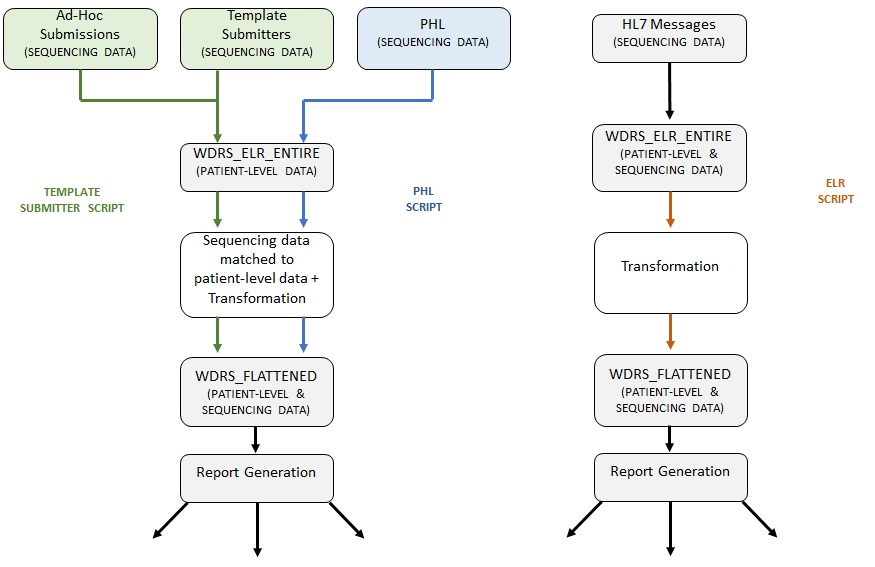
\includegraphics{assets/overview.jpg}

}

\caption{\label{fig-overview}Overview of sequencing pipeline}

\end{figure}%

In addition to sequencing data submissions and WDRS, there is a third
component; GISAID (Global Initiative on Sharing Avian Influenza Data).
GISAID is an initiative that provides open-access to genomic data of
influenza viruses and more importantly for the purposes of this project,
SARS-CoV-2; coronavirus responsible for the COVID-19 pandemic). This
database is available online to the public and holds genomic data of
sequenced specimens from across the globe. In theory, submitters should
be sending their sequencing data to the DOH and GISAID. When this
happens there is consistency between both databases and the data
received from submitters Figure~\ref{fig-gisaid}

\begin{figure}[H]

\centering{

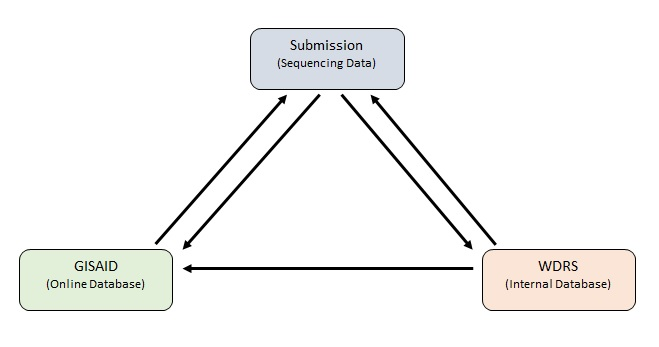
\includegraphics{assets/gisaidflow.jpg}

}

\caption{\label{fig-gisaid}Sequence submissions should match WDRS and
GISAID}

\end{figure}%

It should be noted that in some instances sequencing data is manually
entered by creating events within WDRS. However, this practice is not
common and generally should be avoided if at all possible in order to
prevent non-standard entries and potential data quality issues.

\subsection{Laboratories and
Submitters}\label{laboratories-and-submitters}

Through various contracts and collaboration with external agencies the
DOH receives sequencing data from numerous submitters. Laboratories are
the entities which perform the sequencing. Submitters are the entities
that relay/send sequencing data to the DOH. Many of our submitters
perform both the sequencing and submission of data. There are some
submitters that send sequencing data to the DOH on behalf of multiple
laboratories as well. Therefore, some laboratories that perform the
sequencing do not directly submit the sequencing data themselves. Data
quality is a significant issue across all submission routes listed
below. This is mainly due to the fact that there are no national
standards as how sequencing data should be transmitted.

\subsection{External Dependencies and Data
Pulls}\label{external-dependencies-and-data-pulls}

Prior to any processing of sequencing data received from submitters
there are numerous data pulls and external dependencies that must be
completed. Below is a brief description of each process
Figure~\ref{fig-pulls}.

\begin{figure}[H]

\centering{

\captionsetup{labelsep=none}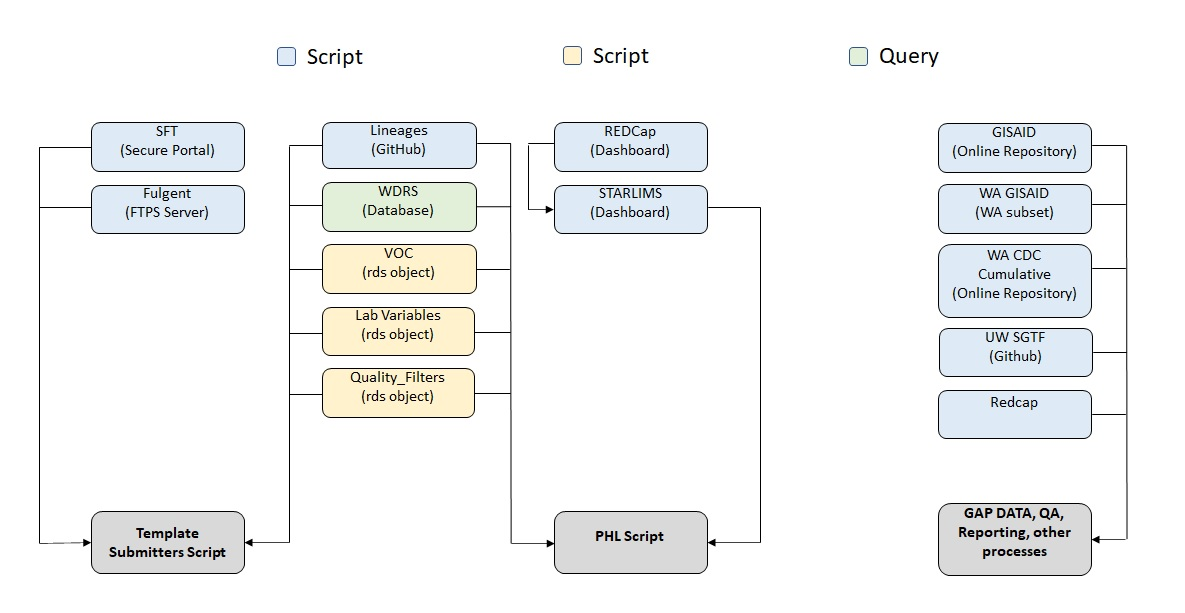
\includegraphics{assets/external_pulls.jpg}

}

\caption{\label{fig-pulls}}

\end{figure}%

The scripts below are responsible for pulling submissions from their
corresponding locations and dropping a file into the submissions folder
in the Network Drive so that it can be picked up by the roster scripts
and processed into WDRS.

\subsubsection{Data Pulls}\label{data-pulls}

\textbf{sel\_Dashboard\_All.Rmd}~performs the task of pulling data from
across three separate dashboard within starLIMS. This data is aggregated
then placed into the submission folder for PHL in the network drive for
processing.

\textbf{sft\_main.py} performs the task of pulling all data from the
individual submitter folders within the SFT, routing the downloaded
files to the correct submitter folders in the network drive, deleting
out the old files, and keeping a log. Additionally, an email is sent out
to the correct stakeholders each day on what submission were uploaded to
the SFT (if any) and notifies of any new labs that have uploaded a
submission for the first time.

\subsubsection{External Processes}\label{external-processes}

\textbf{wa\_cdc\_pull.Rmd} performs the task of pulling data from the
CDC for specimens sequenced by laboratories under the CDC for the state
of Washington so that it can be picked up by multiple QA scripts and
utilized by other other stakeholders.

\textbf{lineages\_main.py} performs the task of pulling data from a .txt
in a GitHub repository containing the latest Covid Lineages and dropping
them in the lineages folder in the network drive so that it can be
picked up by multiple scripts and utilized by other stakeholders. The
.txt file in the repository is the same file used update the
Cov-Lineages site (\url{https://cov-lineages.org/lineage_list.html}).

\paragraph{SGTF}\label{sgtf}

To assist with the monitoring of Omicron, five labs are submitting
S-gene target failures (SGTF) data to WADOH via Redcap or GitHub (UW
only). These submissions are standardized and compiled each day to
calculate \% SGTF by epidemiological week.

\textbf{sgtf\_compile\_daily.Rmd} performs the task of compiling all the
templates and performing the necessary calculations. Submissions are
downloaded by Molecular Epi each day and placed into the network drive
to be picked up by sgtf\_compile\_daily.Rmd

\textbf{uw\_sgtf.Rmd} performs the task of pulling the latest SGTF file
from UW's GitHub repository, routing the downloaded files to the correct
folder in the Network Drive, and keeping a log.

\subsection{Example Datasets}\label{example-datasets}

In 2021, data was sent from sequencing labs to us via tabular files.
There were no standards between submitting labs, and for a given
submitter the format of the tabular files would often change between
each submission as well\hspace{0pt}. It was impossible to process these
data without editing scripts each time to account for a varying format.
Initially, all data was received via non-standardized tabular files,
including data sent from our public health lab (PHL). We did not have
access to their starLIMS database at the time. Table~\ref{tbl-tabdata1}
below is an example of the data sent to us in tabular format.
Table~\ref{tbl-tabdata2} shows data sent in tabular form from our public
health laboratory (PHL) and Table~\ref{tbl-tabdata3} is an example of
data sent from the University of Washington Virology Lab (UW Virology).

\begin{longtable}[]{@{}
  >{\raggedright\arraybackslash}p{(\columnwidth - 2\tabcolsep) * \real{0.3194}}
  >{\raggedright\arraybackslash}p{(\columnwidth - 2\tabcolsep) * \real{0.6806}}@{}}
\caption{example of tabular datasets sent to the Department of Health
from sequencing labs in 2021}\label{tbl-tabdata1}\tabularnewline
\toprule\noalign{}
\begin{minipage}[b]{\linewidth}\raggedright
Variable
\end{minipage} & \begin{minipage}[b]{\linewidth}\raggedright
Description
\end{minipage} \\
\midrule\noalign{}
\endfirsthead
\toprule\noalign{}
\begin{minipage}[b]{\linewidth}\raggedright
Variable
\end{minipage} & \begin{minipage}[b]{\linewidth}\raggedright
Description
\end{minipage} \\
\midrule\noalign{}
\endhead
\bottomrule\noalign{}
\endlastfoot
Accession & identifier that links a sequence to a test \\
COLLECTION\_SAMPLE\_ID & the identifier that linked a sequence to a
test \\
ORIG\_ACCESSION\_NUMBER & the identifier that linked a sequence to a
test \\
PAT\_FIRST\_NAME & patient first name \\
PAT\_LAST\_NAME & patient last name \\
DATE\_OF\_BIRTH & date of birth \\
PAT\_ADDRESS\_1 & address \\
PAT\_CITY & city \\
PAT\_STATE & state \\
PAT\_ZIP & zip code \\
Phone & phone number \\
Original Physician & doctor name \\
\end{longtable}

\begin{longtable}[]{@{}
  >{\raggedright\arraybackslash}p{(\columnwidth - 2\tabcolsep) * \real{0.3611}}
  >{\raggedright\arraybackslash}p{(\columnwidth - 2\tabcolsep) * \real{0.6389}}@{}}
\caption{example of tabular datasets sent to the Department of Health
from a Public Health Lab (PHL) during
2021}\label{tbl-tabdata2}\tabularnewline
\toprule\noalign{}
\begin{minipage}[b]{\linewidth}\raggedright
Variable
\end{minipage} & \begin{minipage}[b]{\linewidth}\raggedright
Description
\end{minipage} \\
\midrule\noalign{}
\endfirsthead
\toprule\noalign{}
\begin{minipage}[b]{\linewidth}\raggedright
Variable
\end{minipage} & \begin{minipage}[b]{\linewidth}\raggedright
Description
\end{minipage} \\
\midrule\noalign{}
\endhead
\bottomrule\noalign{}
\endlastfoot
LIMS & the laboratory information management system (LIMS) \\
Project & the reason for sequencing \\
Investigator\_sample\_id & an identifier to the sample \\
collection\_date & the specimen collection date \\
age & patient age \\
county & patient county \\
sex & patient sex \\
specimen\_id & the identifier linking to the original PCR covid test \\
submitting\_lab & the lab submitting the sequence \\
note & free text note field \\
\end{longtable}

\begin{longtable}[]{@{}
  >{\raggedright\arraybackslash}p{(\columnwidth - 2\tabcolsep) * \real{0.3611}}
  >{\raggedright\arraybackslash}p{(\columnwidth - 2\tabcolsep) * \real{0.6389}}@{}}
\caption{example of tabluar datasets sent to the Department of Health by
UW Virology during 2021}\label{tbl-tabdata3}\tabularnewline
\toprule\noalign{}
\begin{minipage}[b]{\linewidth}\raggedright
Variable
\end{minipage} & \begin{minipage}[b]{\linewidth}\raggedright
Description
\end{minipage} \\
\midrule\noalign{}
\endfirsthead
\toprule\noalign{}
\begin{minipage}[b]{\linewidth}\raggedright
Variable
\end{minipage} & \begin{minipage}[b]{\linewidth}\raggedright
Description
\end{minipage} \\
\midrule\noalign{}
\endhead
\bottomrule\noalign{}
\endlastfoot
uwnum & the identifier of the sequence that links to GISAID \\
acc\_num & the accession number linking to the positive covid PCR
test \\
collection date & specimen collection date \\
loc\_state & patient state \\
fullname & the full GISAID identifier name, such as
HCoV19-USA/WA-\#\#\#\#\#/2021 (not the patient's name) \\
shortname & a partial GISAID identifier name, such as
WA-\#\#\#\#\#\#\# \\
\end{longtable}

As you can see from the tables above, data sent via tabular format early
in the project was not standardized and could not be processed
automatically due to it constantly changing field names and
descriptions.

\section{Roster Workflows}\label{roster-workflows}

There are three main workflows for rostering sequencing data into WDRS.
\href{@sec-elr}{ELR}, \href{@sec-phl}{PHL}, and
\href{@sec-template}{Template} scripts as detailed in
Section~\ref{sec-overview}. All three will output a roster, and the
\href{@sec-rostercompile}{Roster Compile} script will combine them and
send the data to be rostered into WDRS. See Figure~\ref{fig-roster} for
a high level overview. The \href{notebooks/elr.Rmd}{elr.Rmd} script
pulls sequencing metadata from WDRS, transforms it, and runs QA checks
on it before putting it into a usable roster.
\href{notebooks/template_submitters.Rmd}{template\_submitters.Rmd}
performs the task of processing template submission.
\href{notebooks/phl.Rmd}{PHL.Rmd} performs the task of processing all
phl records. Both the template and phl processes operate based on
similar logic from a high level view, but there are significant
differences between each script.

The \texttt{SEQUENCE\_CLINICAL\_ACCESSION} variable is used to find a
matching event within the \texttt{{[}dbo{]}.{[}DD\_ELR\_DD\_ENTIRE{]}}
table. The \texttt{CASE\_ID} (WDRS variable that is an identifier for a
disease case, not a person) for that event is pulled then assigned to
the corresponding record. At this point, if an event using the accession
ID cannot be found for a record it will be routed to two different
processes depending on if the sequencing data received has patient
demographics attached to it; FIRST\_NAME, LAST\_NAME, MIDDLE\_NAME, DOB.
If the record received contains patient demographic it is routed to the
\href{notebooks/fuzzy.Rmd}{fuzzy matching process}, an attempt to match
to the correct event will be made using the demographic information. If
the record received contains no patient demographic it is routed to the
keep na process (Section~\ref{sec-keepna}), the record will be retained
and an attempt to match via the accession ID will regularly be made in
case the corresponding event populates in WDRS later on.

Once a record has been matched to an event it will undergo
transformation to clean and standardize the matched data into a roster
format. Some submitters do not provide the full \texttt{GISAID\_ID} in
the submission. In this case, the \texttt{SEQUENCE\_ACCESSION} can be
constructed from their internal accession is inputted into the
\texttt{GISAID\_ID} column. This happens during the transformation
process and the resulting \texttt{SEQUENCE\_ACCESSION} should match to
what is in GISAID.

Records are then put through a series of quality filters to check for QA
issues. All records that pass this series of QA checks will then
populated into a final roster then outputted to be picked up by the
roster compile script Section~\ref{sec-rostercompile} and sent to data
support for upload to WDRS.

\begin{figure}[H]

\centering{

\captionsetup{labelsep=none}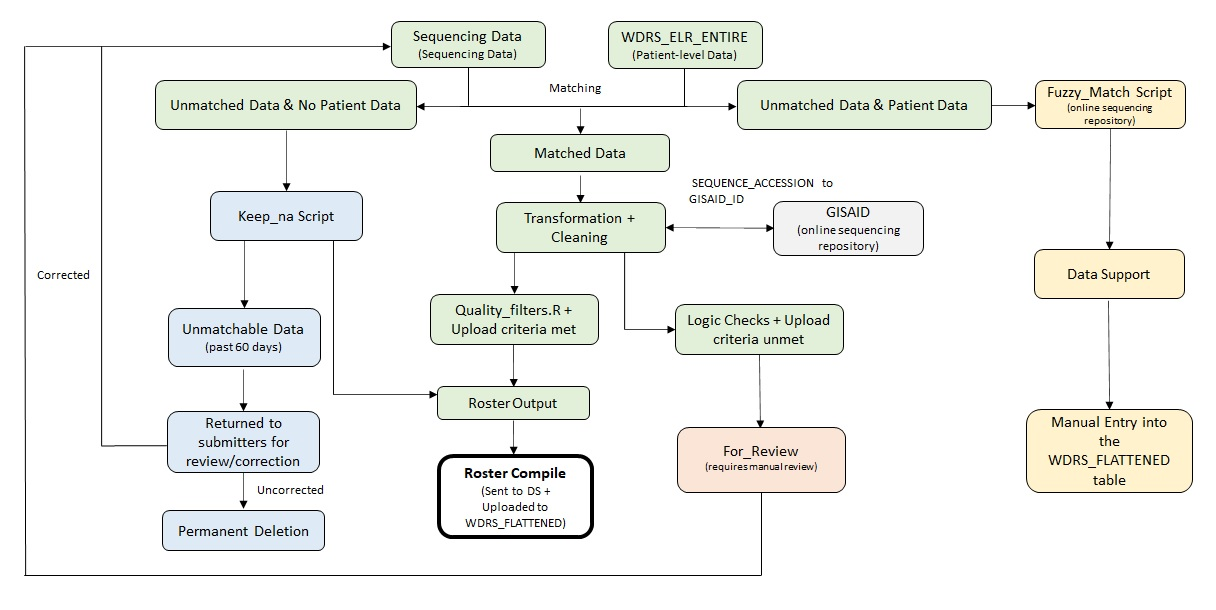
\includegraphics{assets/roster.jpg}

}

\caption{\label{fig-roster}}

\end{figure}%

\subsection{Roster Scripts}\label{sec-ecosystem}

This section gives more details about each roster script and a high
level diagram following the process.\\

Legend:


\includegraphics[width=4.27in,height=0.51in]{index_files/figure-latex/mermaid-figure-18.png}

\textsubscript{Source:
\href{https://NW-PaGe.github.io/sequencing_integration_pipeline1.0/index.qmd.html}{Article
Notebook}}

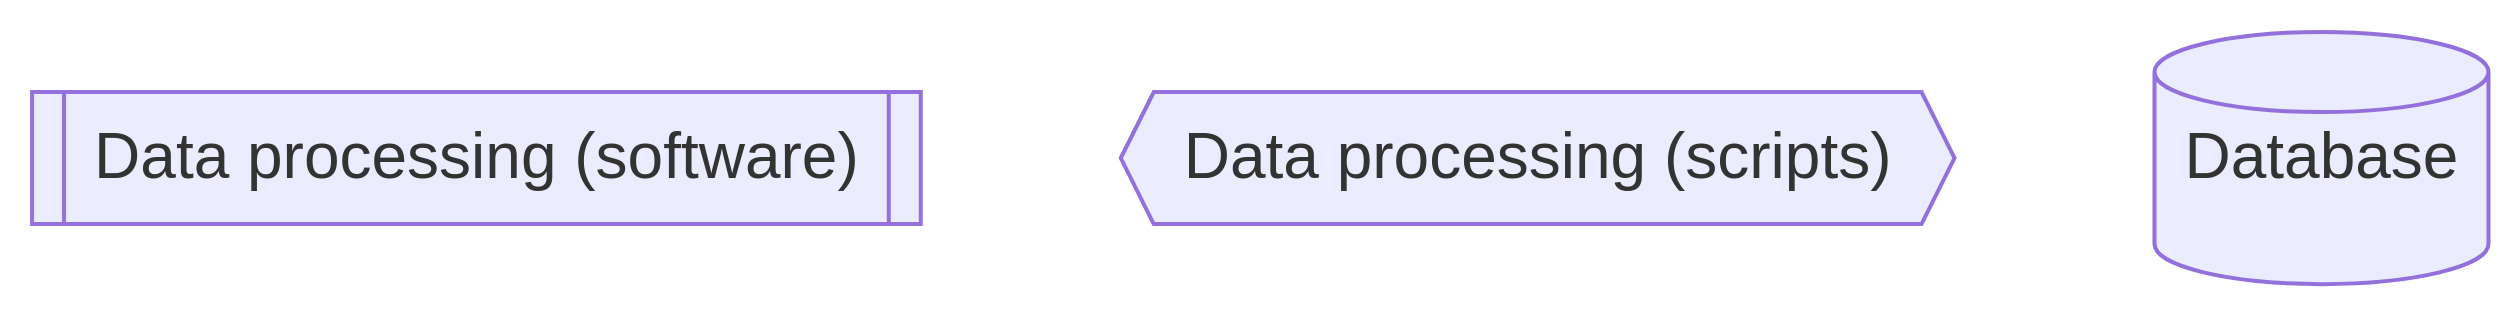
\includegraphics[width=6.56in,height=0.82in]{index_files/figure-latex/mermaid-figure-17.png}

\textsubscript{Source:
\href{https://NW-PaGe.github.io/sequencing_integration_pipeline1.0/index.qmd.html}{Article
Notebook}}

\subsubsection{ELR}\label{sec-elr}

Electronic Lab Reporting for sequencing went live in September 2021.
These are records with Covid PCR tests processed by WELRS/DRIVE and sent
to WDRS\hspace{0pt}. See Figure~\ref{fig-elrflow} below. For more
details on the script, see \href{notebooks/elr.Rmd}{the ELR notebook}.
From a high-level overview, the script will:

\begin{itemize}
\tightlist
\item
  WELRS/DRIVE process, match, and fill the entire/lab tables but not
  sequencing table\hspace{0pt}
\item
  No QA processing\hspace{0pt}
\item
  Sequencing table is built as an after thought\hspace{0pt}
\item
  WELRS/DRIVE is somewhat of a black box to us (changes without
  knowing,~don't have oversight on mismatches)\hspace{0pt}
\item
  Our ELR script will extract from the entire table, transform, QA, and
  send via~roster\hspace{0pt}
\end{itemize}

\begin{figure}[H]

\centering{

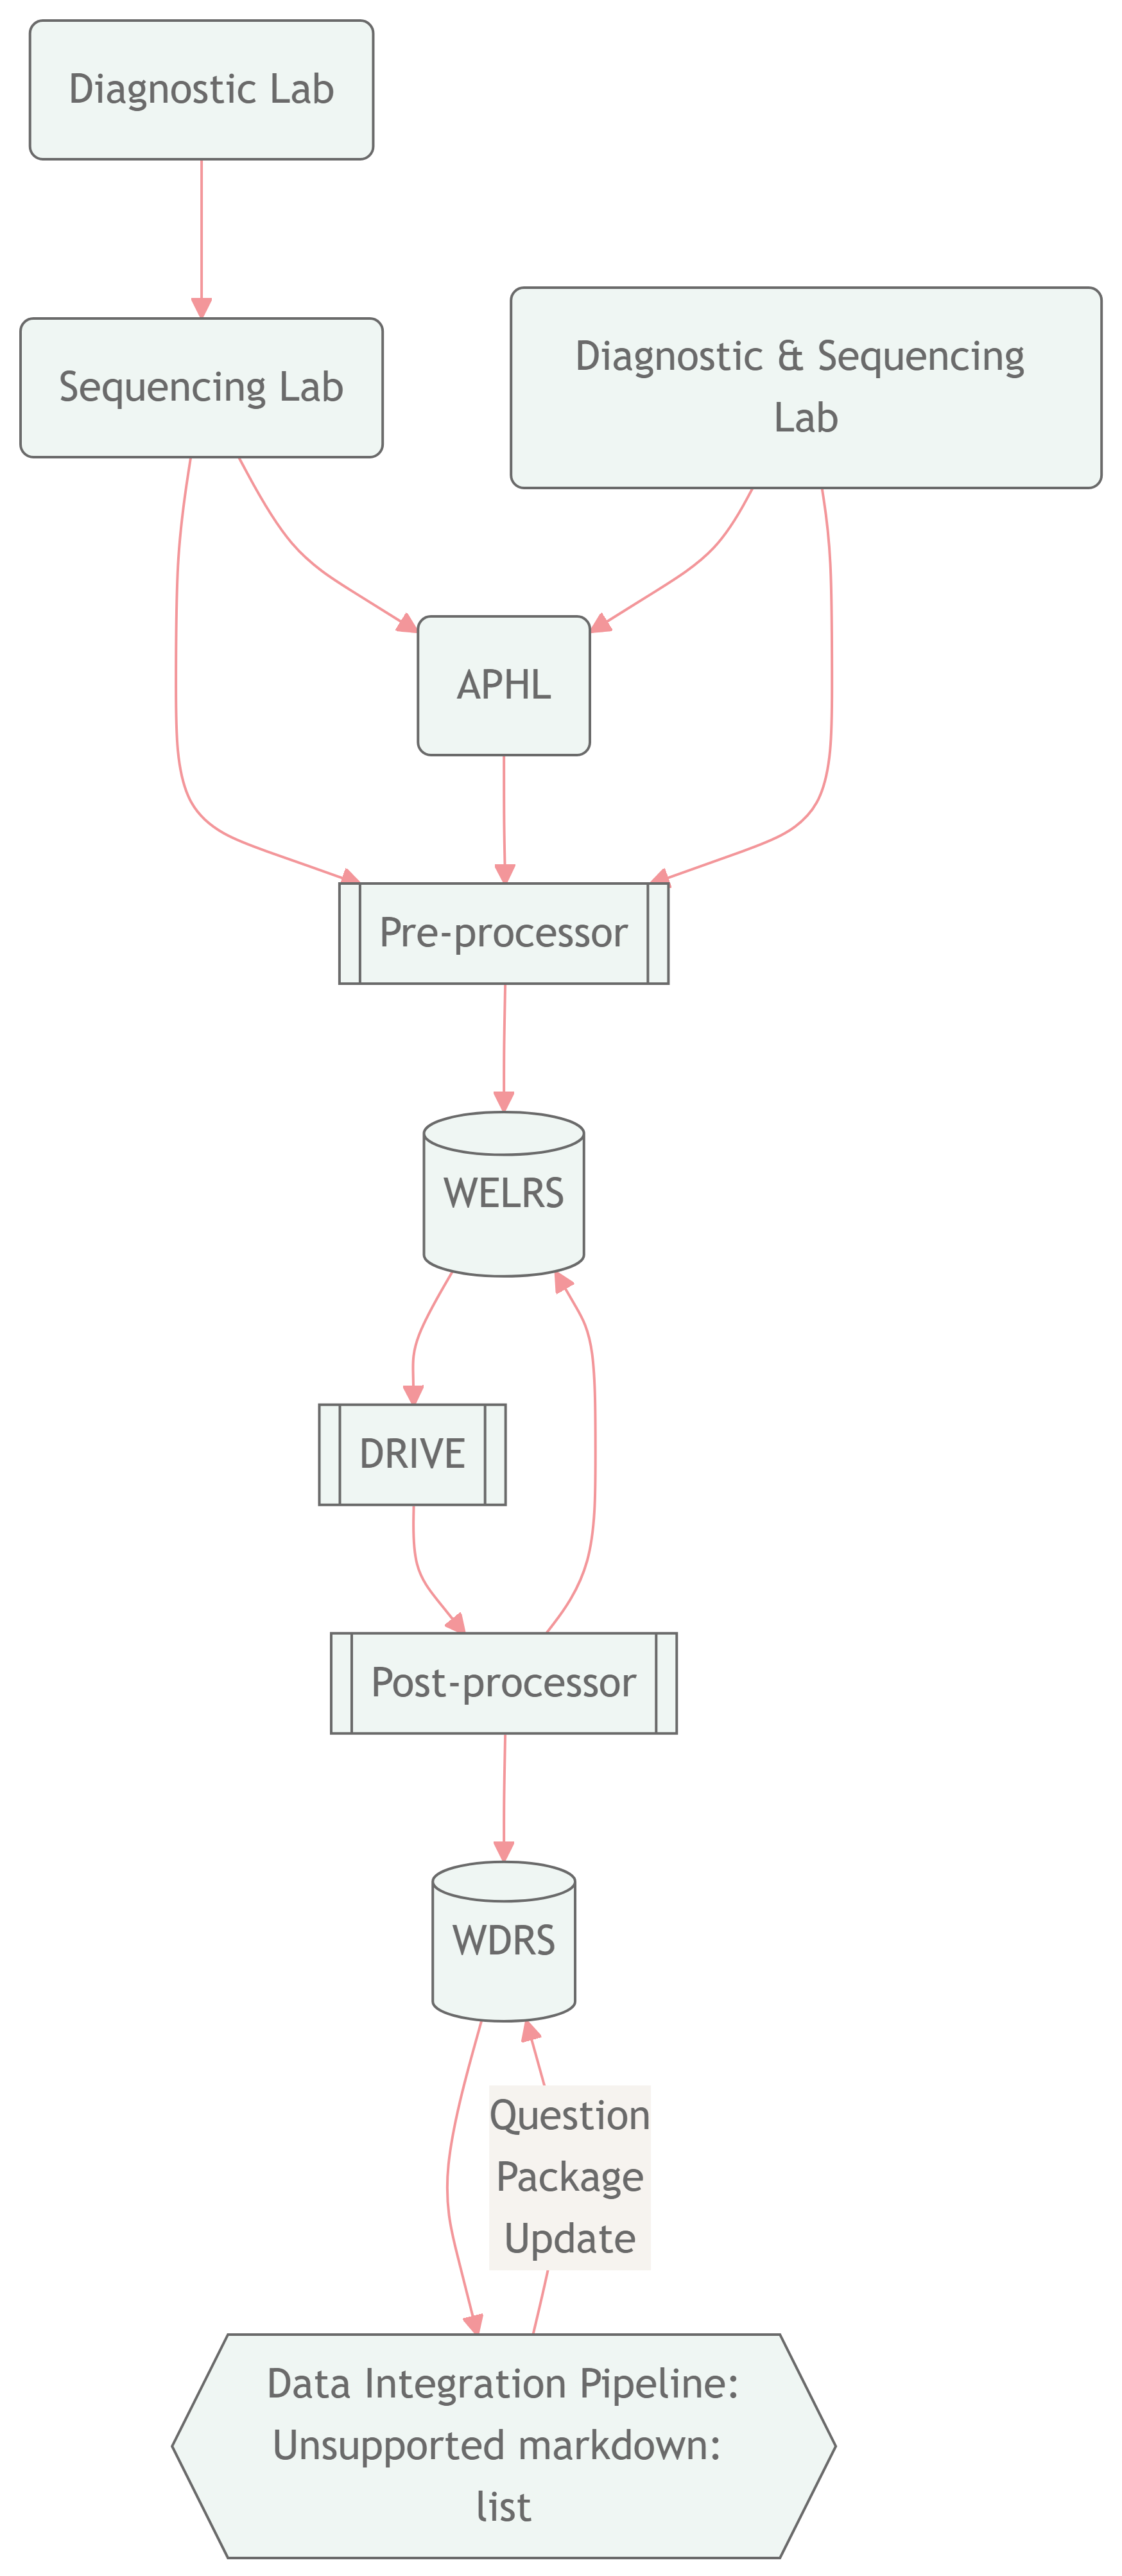
\includegraphics[width=3in,height=6.22in]{index_files/figure-latex/mermaid-figure-16.png}

}

\caption{\label{fig-elrflow}ELR submission to WDRS workflow}

\end{figure}%

\textsubscript{Source:
\href{https://NW-PaGe.github.io/sequencing_integration_pipeline1.0/index.qmd.html}{Article
Notebook}}

\subsubsection{PHL}\label{sec-phl}

Access to starLIMS, our Public Health Laboratory (PHL) system, was
granted in April 2021. However, there was no API or underlying database
access so the pipeline needed to scrape data from the starLIMS
dashboard. It would download the \texttt{.xslx} files from starLIMS and
then use identifiers to match sequences to a case in our database, WDRS.
See Figure~\ref{fig-phlflow} below for a high level summary. This
process can get complicated for a multitude of reasons mainly due to
challenges with our underlying data infrastructure. For more details on
the workflow and to view those challenges, see
\href{notebooks/phl.Rmd\#fig-phlworkflow}{more details here} and for all
script details see \href{notebooks/phl.Rmd}{the PHL notebook}. From a
high-level overview, the script will:

\begin{itemize}
\tightlist
\item
  Scrape from StarLIMS\hspace{0pt}
\item
  Match to a WDRS case~\hspace{0pt}
\item
  If no match based on \texttt{FILLER\_ORDER\_NUM}~then match
  on~demographics\hspace{0pt}
\item
  Uses a processed file to eliminate feedback loops (prevent failed
  records from being processed every run)\hspace{0pt}
\item
  Fields may change in starLIMS without our knowledge\hspace{0pt}
\end{itemize}

\begin{figure}[H]

\centering{

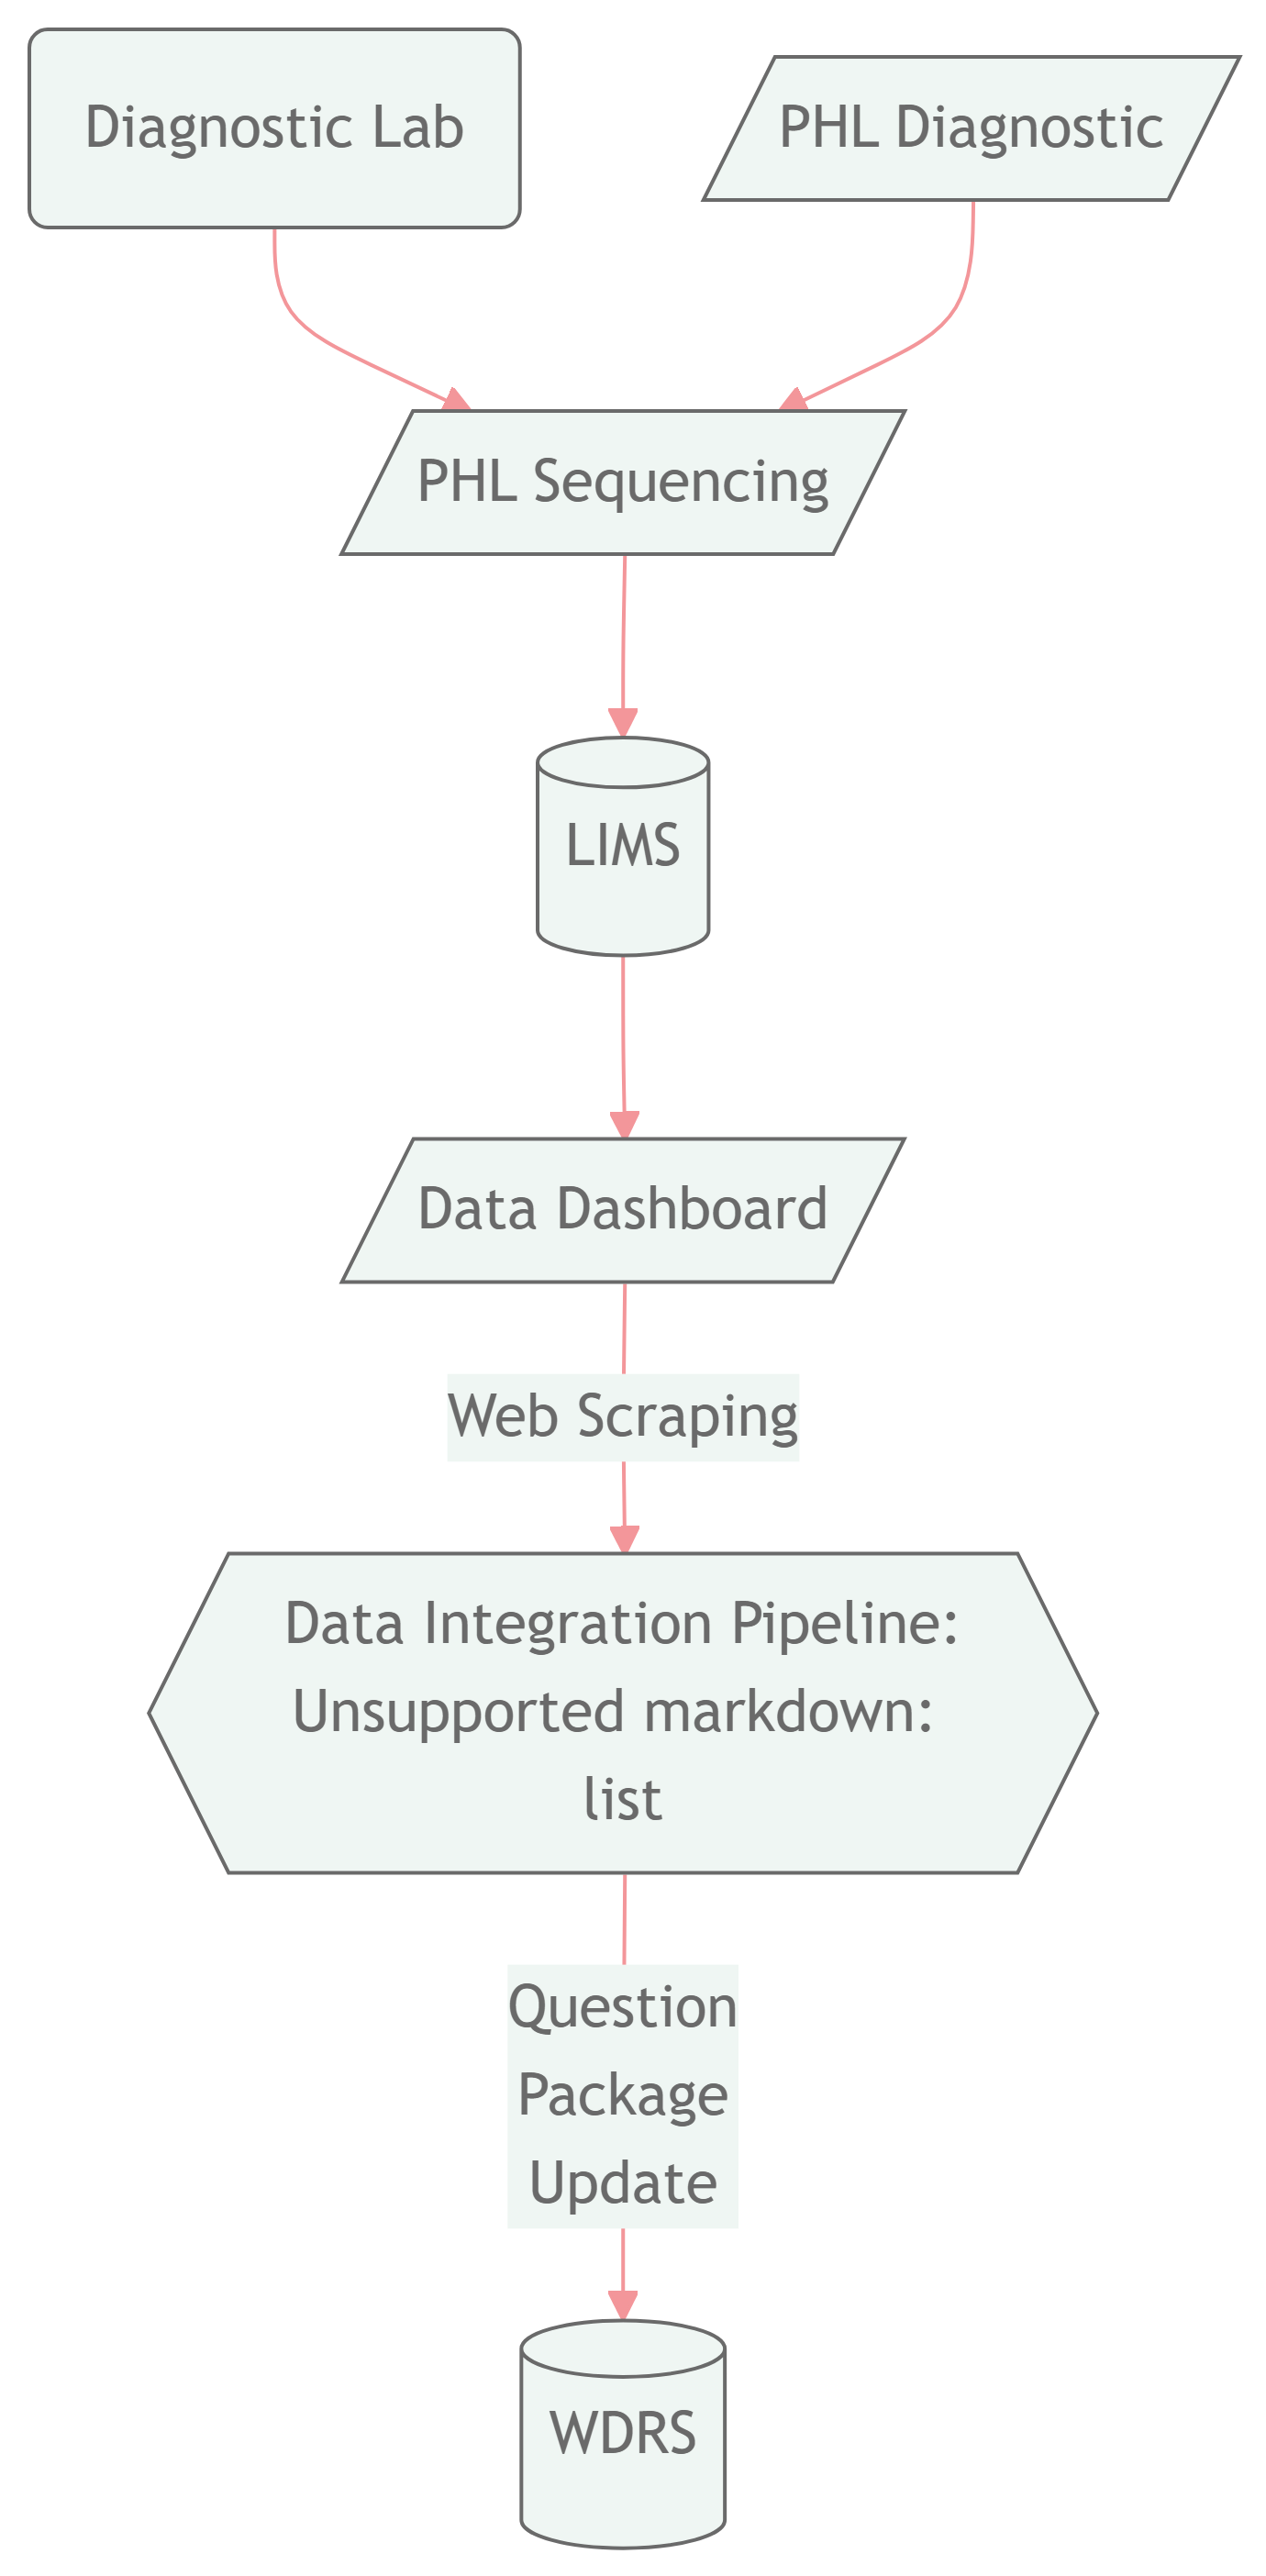
\includegraphics[width=3in,height=5.59in]{index_files/figure-latex/mermaid-figure-15.png}

}

\caption{\label{fig-phlflow}PHL submission to WDRS workflow}

\end{figure}%

\textsubscript{Source:
\href{https://NW-PaGe.github.io/sequencing_integration_pipeline1.0/index.qmd.html}{Article
Notebook}}

\subsubsection{Template}\label{sec-template}

There are still labs that cannot send us data via ELR or PHL and could
only send us tabular files. The Department of Health has a secure file
transfer (SFT) site that the labs could send data to and that we could
pull from. We did not have a way to pull from our own SFT site so we
needed to scrape this data as well. In July 2021, Cory Yun developed a
template (see Table~\ref{tbl-template}) for labs to fill the sequencing
data instead of labs sending us data with no standards. See
Figure~\ref{fig-templateflow} below. For script details see
\href{notebooks/template_submitters.Rmd}{the template submitters
notebook}. From a high-level overview, the script will:

\begin{itemize}
\tightlist
\item
  Labs send us a \texttt{.csv} file into our MFT site\hspace{0pt}
\item
  All data follows a specific template created by Cory\hspace{0pt}
\item
  Scrape the site and download the \texttt{.csv} files for each
  lab\hspace{0pt}
\item
  Format, find a match based on \texttt{FILLER\_ORDER\_NUM} or
  demographics
\end{itemize}

\begin{longtable}[]{@{}
  >{\raggedright\arraybackslash}p{(\columnwidth - 4\tabcolsep) * \real{0.4028}}
  >{\raggedright\arraybackslash}p{(\columnwidth - 4\tabcolsep) * \real{0.3472}}
  >{\raggedright\arraybackslash}p{(\columnwidth - 4\tabcolsep) * \real{0.2500}}@{}}
\caption{Template Data Variables}\label{tbl-template}\tabularnewline
\toprule\noalign{}
\begin{minipage}[b]{\linewidth}\raggedright
Variable
\end{minipage} & \begin{minipage}[b]{\linewidth}\raggedright
Description
\end{minipage} & \begin{minipage}[b]{\linewidth}\raggedright
Example
\end{minipage} \\
\midrule\noalign{}
\endfirsthead
\toprule\noalign{}
\begin{minipage}[b]{\linewidth}\raggedright
Variable
\end{minipage} & \begin{minipage}[b]{\linewidth}\raggedright
Description
\end{minipage} & \begin{minipage}[b]{\linewidth}\raggedright
Example
\end{minipage} \\
\midrule\noalign{}
\endhead
\bottomrule\noalign{}
\endlastfoot
LAB\_ACCESSION\_ID & id matching a sequence to a PCR test & alphanumeric
string \\
GISAID\_ID & identifier of sequence in GISAID & USA/WA-X/2020 \\
SPECIMEN\_COLLECTION\_DATE & collection date of specimen & mm-dd-yyyy \\
SUBMITTING\_LAB & lab name & UW Virology \\
SEQUENCE\_REASON & reason for sequencing & SENTINEL SURVEILLANCE \\
SEQUENCE\_STATUS & complete or failed sequence & COMPLETE \\
PANGO\_LINEAGE & lineage call in GISAID & BA.1 \\
FIRST\_NAME & patient first name & \\
LAST\_NAME & patient last name & \\
MIDDLE\_NAME & patient middle name & \\
DOB & date of birth & \\
ALTERNATIVE\_ID & alternative identifier & alphanumeric string \\
\end{longtable}

\begin{figure}[H]

\centering{

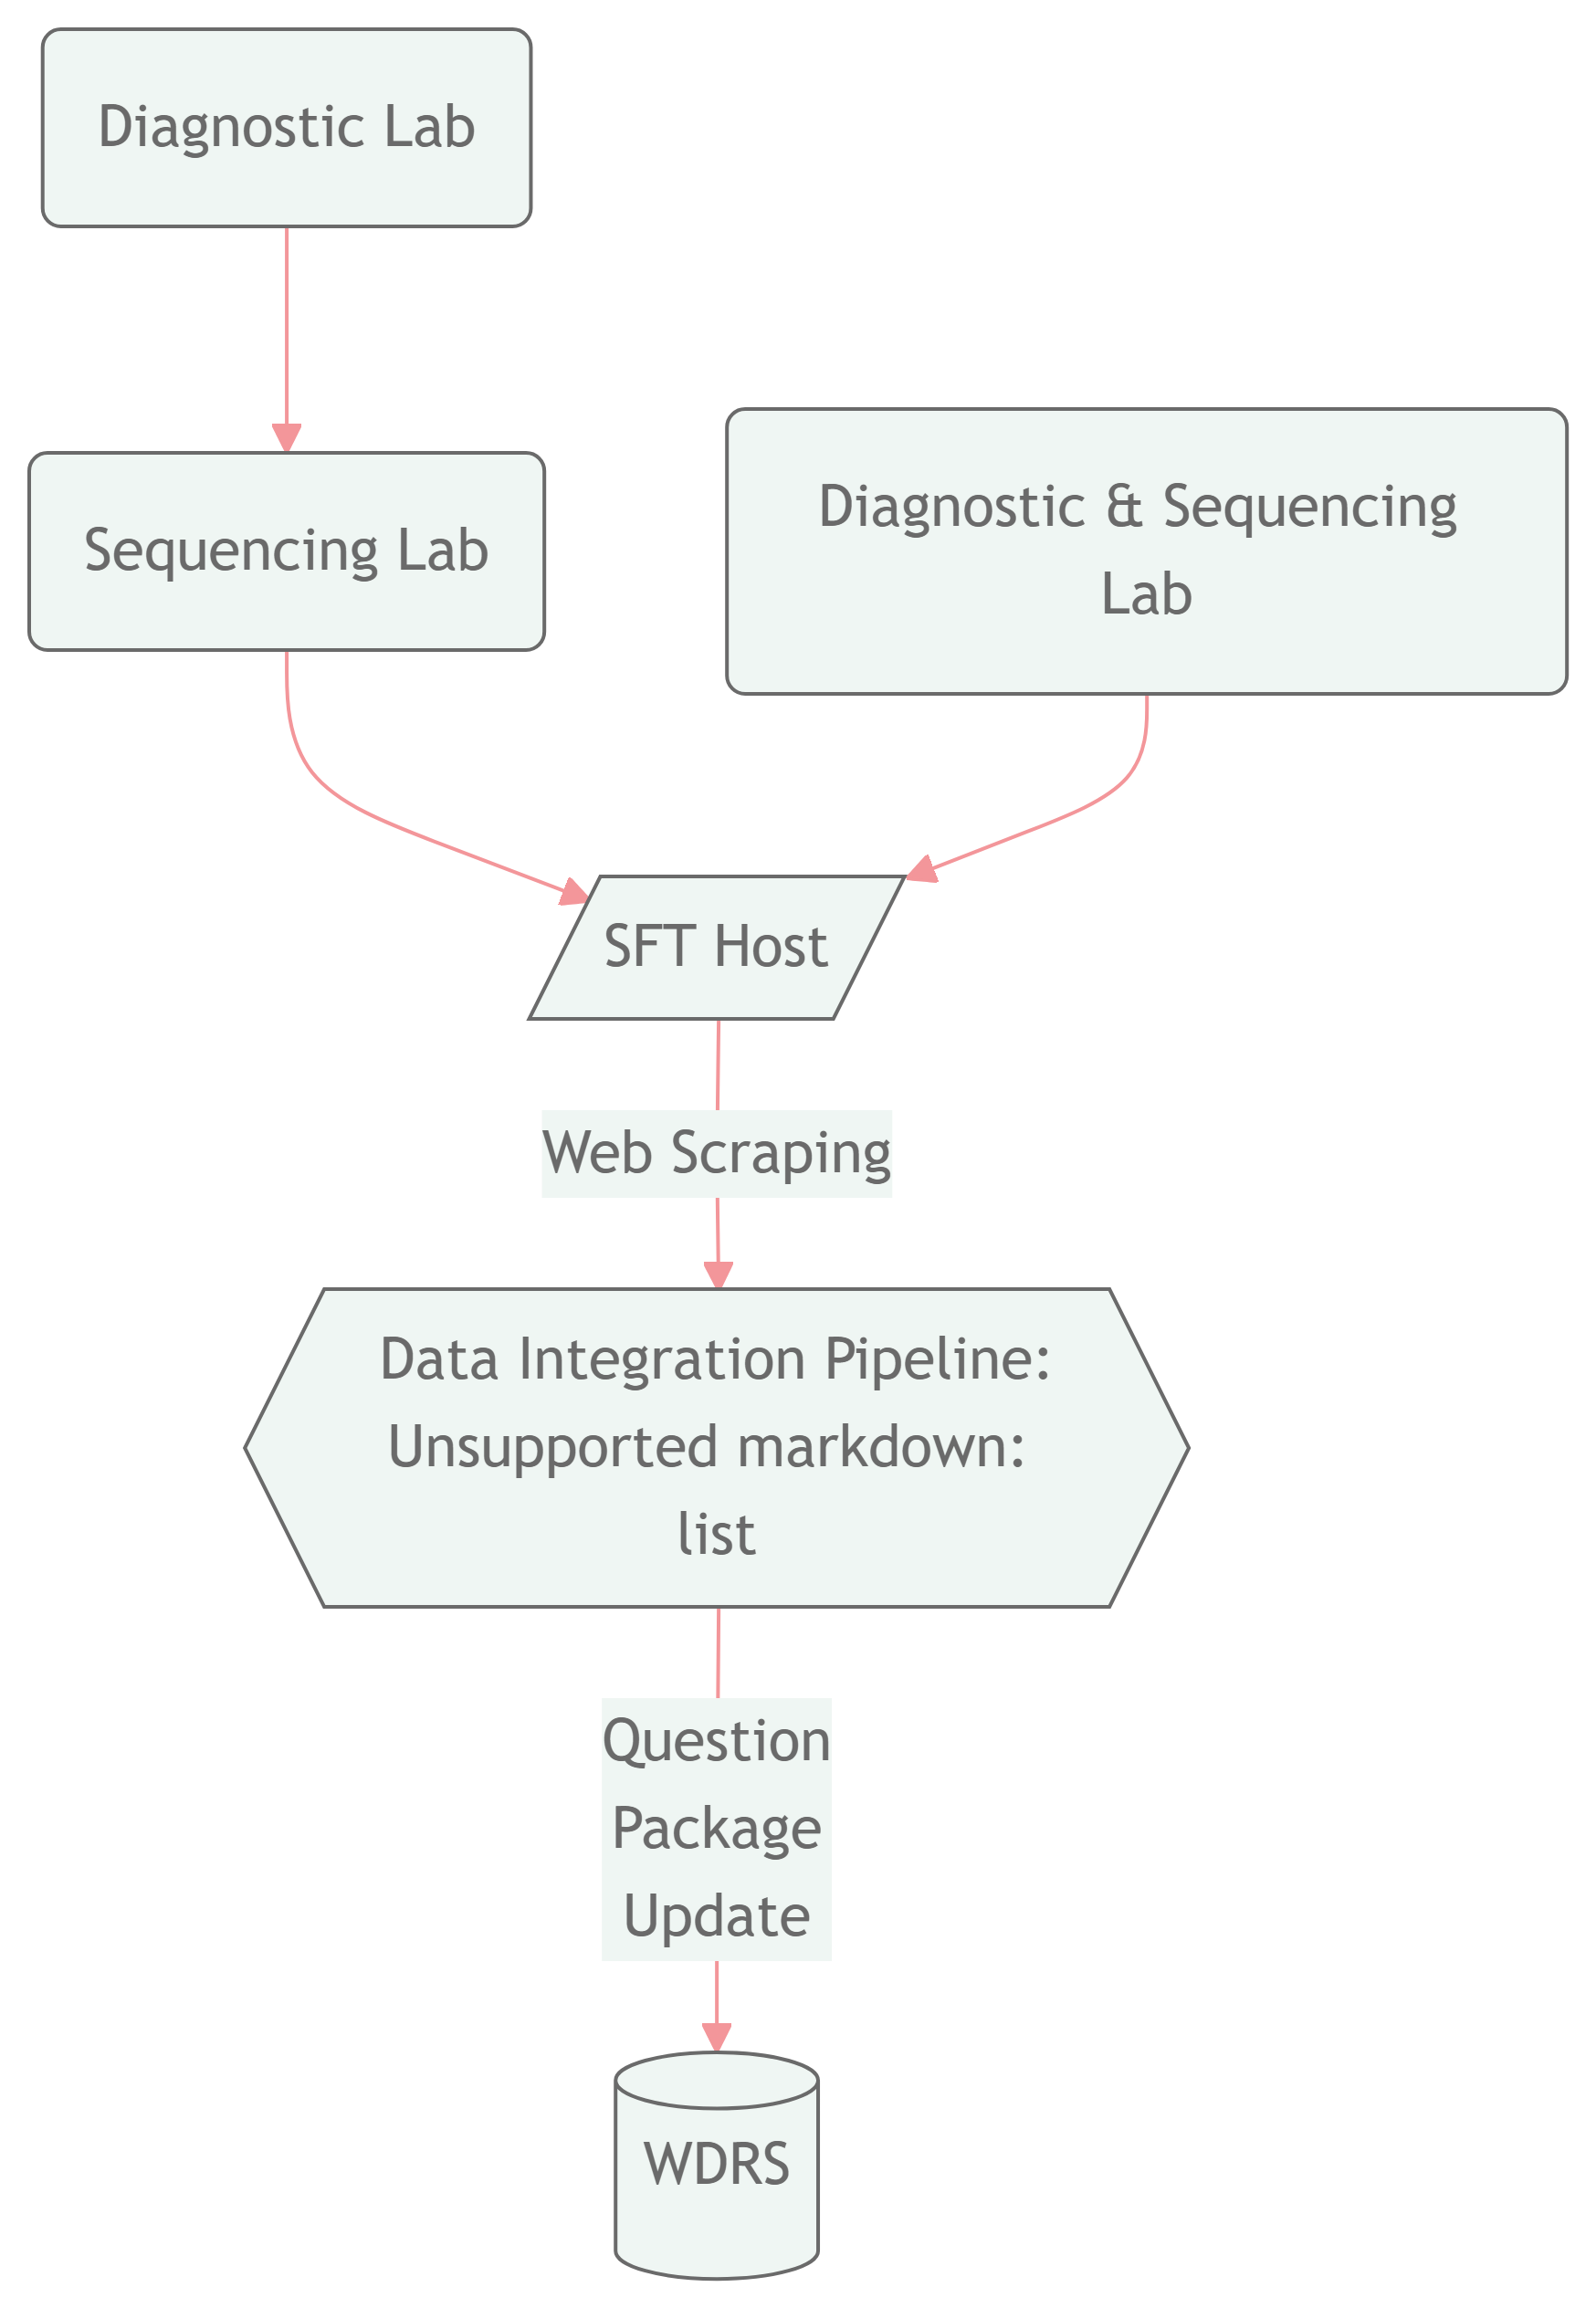
\includegraphics[width=3in,height=3.92in]{index_files/figure-latex/mermaid-figure-14.png}

}

\caption{\label{fig-templateflow}Template submission to WDRS workflow}

\end{figure}%

\textsubscript{Source:
\href{https://NW-PaGe.github.io/sequencing_integration_pipeline1.0/index.qmd.html}{Article
Notebook}}

\subsubsection{Roster Compile}\label{sec-rostercompile}

After the Template, PHL, and ELR scripts run, they all output a
\texttt{.csv} file into a folder called \texttt{write\_roster\_here} in
our network drive. The \href{ROSTER_COMPILE.Rmd}{Roster Compile} script
reads in all of these files, combines them, and runs additional QA
checks on them before outputting the results into one file for output to
the WDRS database. Then our Data Support team will upload the file into
WDRS where it will update the results into the flattened table. Each row
will match a \texttt{CASE\_ID} in WDRS and the sequencing event is added
to the cases external data as seen below in
Figure~\ref{fig-examplewdrs}.

\begin{figure}[H]

\centering{

\captionsetup{labelsep=none}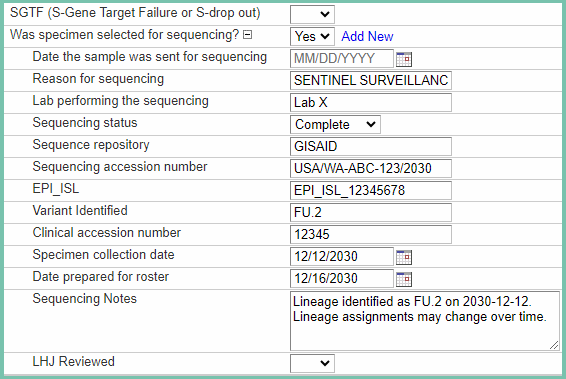
\includegraphics{assets/example_qp_frontend.png}

}

\caption{\label{fig-examplewdrs}}

\end{figure}%

\subsection{For Review}\label{for-review}

The pipeline attempts to link sequencing data to cases in WDRS. Some
records have quality issues and cannot be processed in our system. These
data are tagged and saved in a separate folder where our team reviews
them and attempts to fix and re-process them. Table~\ref{tbl-review} is
an example of the sort of issues that get tagged in our pipeline:

\begin{longtable}[]{@{}
  >{\raggedright\arraybackslash}p{(\columnwidth - 2\tabcolsep) * \real{0.5000}}
  >{\raggedright\arraybackslash}p{(\columnwidth - 2\tabcolsep) * \real{0.5000}}@{}}
\caption{For review quality issue tags}\label{tbl-review}\tabularnewline
\toprule\noalign{}
\begin{minipage}[b]{\linewidth}\raggedright
Variable
\end{minipage} & \begin{minipage}[b]{\linewidth}\raggedright
Description
\end{minipage} \\
\midrule\noalign{}
\endfirsthead
\toprule\noalign{}
\begin{minipage}[b]{\linewidth}\raggedright
Variable
\end{minipage} & \begin{minipage}[b]{\linewidth}\raggedright
Description
\end{minipage} \\
\midrule\noalign{}
\endhead
\bottomrule\noalign{}
\endlastfoot
QA\_CASE\_ID & Missing CASE\_ID from WDRS \\
QA\_SCA\_NA & Clinical Accession identifier is missing \\
QA\_SCA\_INT\_DUPE & Clinical Accession duplicate in file \\
QA\_SCA\_WDRS\_DUPE & Clinical Accession duplicate found in WDRS \\
QA\_SA\_INT\_DUPE & Accession duplicate in file \\
QA\_SA\_WDRS\_DUPE & Accession duplicate found in WDRS \\
QA\_SEQ\_VARIANT & Variant not in list of VOC \\
QA\_SEQ\_STAT & Status error (labeled complete sequence when it was
failed) \\
QA\_SEQ\_REASON & Unknown sequence reason \\
QA\_SEQ\_NOTES & Sequence note not formatted \\
QA\_COLLECT\_DATE & Match found but collection dates \textgreater14
days \\
QA\_OTHER & Other formatting issues \\
sum & Total number of errors found \\
\end{longtable}

\subsection{Fuzzy Matching Review}\label{fuzzy-matching-review}

When records cannot be linked via accession identifier the pipeline
attempts to match a sequence to a PCR test in WDRS via demographics
(first name, last name, date of birth, and collection date). The
\href{notebook/fuzzy.Rmd}{fuzzy matching script} uses
\href{https://github.com/markvanderloo/stringdist}{string distances} to
match names from a submitter to names in WDRS and determine the highest
likelihood of a correct link.

There may be quality issues with the demographics and the fuzzy matching
script tags issues and outputs them into a fuzzy matching review folder
where our team will manually review the errors and re-process the files.
Table~\ref{tbl-fuzzyreview} is an example of the files the fuzzy
matching process outputs:

\begin{longtable}[]{@{}ll@{}}
\caption{Fuzzy matching review quality issue
tags}\label{tbl-fuzzyreview}\tabularnewline
\toprule\noalign{}
File & Description \\
\midrule\noalign{}
\endfirsthead
\toprule\noalign{}
File & Description \\
\midrule\noalign{}
\endhead
\bottomrule\noalign{}
\endlastfoot
Fuzzy bad rows & error in a column other than demographics columns \\
Fuzz 1 & best match was a name levenshtein distance of 1 \\
Fuzz 2 & best match was a name levenshtein distance of 2 \\
Fuzz 3 & best match was a name levenshtein distance of 3 \\
Did\_not\_match & no match was found \\
Fuzzy perfect & perfect match found \\
\end{longtable}

\subsection{Keep NA}\label{sec-keepna}

A sequenced specimen may not initially match to our database (WDRS) for
many reasons. A case may not have been updated at the time our pipeline
tried to match the sequence to the PCR test, or a sequence may simply
not match to a case in WDRS. Our
\href{KEEP_NA_ROSTER_SECOND_IN_PROGRESS.Rmd}{Keep NA script} reads in
all the data that could not be matched in previous pipeline runs and
attempts to match them again in the case that new and updated case data
is in WDRS. If an unmatched record is in our archive for more than 60
days the Keep NA script will remove it from the list and keep it in an
archived file. We made this decision because the vast majority of
records that are in Keep NA for over 60 days have never matched to any
case in WDRS.

\section{QA Processes}\label{qa-processes}

\subsection{Gap data}\label{gap-data}

\textbf{gap\_data.Rmd} performs the task of identifying and tracking the
number of sequencing records for the state of WA that have been
submitted to GISAID but are missing from WDRS. As previously mentioned,
submitters should be sending records to both the DOH and GISAID. This
process uses the \texttt{SEQUENCE\_ACCESION} (\texttt{GISAID\_ID}) to
identify any records from GISAID that are not in WDRS for the state of
WA. An excel file containing two pivot tables and metadata is output.
Each pivot table contains either the number or proportion of records
missing in WDRS, this information is the submission date (month-year)
and the submitting lab. The metadata contains each record and
accompanying information pulled from GISAID.

This output is utilized by Data Support and other stakeholders for two
main reasons. First, to reach out to submitters to regarding missing
records. Second, to identify any new that are submitting to GISAID
regularly and should potentially be onboarded.

\subsection{WDRS Logic Checks}\label{wdrs-logic-checks}

\texttt{wdrs\_logic\_checks.R} pulls the sequencing data from our
database and runs checks on them to confirm that there are no issues
with the data uploaded. See Table~\ref{tbl-qachecks} below for more
info.

\begin{longtable}[]{@{}
  >{\raggedright\arraybackslash}p{(\columnwidth - 2\tabcolsep) * \real{0.5278}}
  >{\raggedright\arraybackslash}p{(\columnwidth - 2\tabcolsep) * \real{0.4722}}@{}}
\caption{WDRS QA Checks}\label{tbl-qachecks}\tabularnewline
\toprule\noalign{}
\begin{minipage}[b]{\linewidth}\raggedright
QA Check
\end{minipage} & \begin{minipage}[b]{\linewidth}\raggedright
Description
\end{minipage} \\
\midrule\noalign{}
\endfirsthead
\toprule\noalign{}
\begin{minipage}[b]{\linewidth}\raggedright
QA Check
\end{minipage} & \begin{minipage}[b]{\linewidth}\raggedright
Description
\end{minipage} \\
\midrule\noalign{}
\endhead
\bottomrule\noalign{}
\endlastfoot
SEQUENCE\_REASON is NULL & The reason for sequencing is used to
determine sentinel surveillance counts and cannot be null \\
SEQUENCE\_REASON not standardized & If the reason has a typo or
unexpected value \\
SEQUENCE\_VARIANT\_OPEN\_TEXT filled but SEQUENCE\_STATUS is not
COMPLETE & Status must be complete when the variant is filled \\
SEQUENCE\_ACCESSION number NULL but status not FAILED/LOW QUALITY & A
sequence identifier must be provided for complete sequences \\
SEQUENCE\_VARIANT\_OPEN\_TEXT exists but SEQUENCE\_ACCESION number is
null & A sequence identifier must be provided for sequences with lineage
calls \\
SEQUENCE\_VARIANT not of concern/interest - check or update list &
Lineage has a typo or not a variant of concern \\
SEQUENCE\_LAB not standardized - check or update list & The lab name is
not standardized to our database standards \\
SEQUENCE\_SPECIMEN\_COLLECTION\_DATE out of range. Before 1/05/2020 or
after today's date & The sequence collection date is in the future or
before 2020 (invalid) \\
SEQUENCE\_SPECIMEN = `No' but sequencing data attatched & Database
error \\
SEQUENCE\_ACCESSION number and SEQUENCE\_CLINICAL\_ACCESSION numbers
missing & A sequence needs the identifiers attached \\
Unexpected characters in a column & Database or submitter error (usually
typos or wrong value in a column) \\
Lineage found in SEQUENCE\_NOTES but SEQUENCE\_VARIANT\_OPEN\_TEXT is
NULL & Database error \\
SEQUENCE\_STATUS = `Complete' and SEQUENCE\_VARIANT\_OPEN\_TEXT is NULL
& Sequence needs a lineage call if status is complete \\
Duplicate - SCA, SA and Variant duplicated & Duplicate identifier values
found in database \\
\end{longtable}

\section{Results}\label{results}

During the February 2021 to September 2023 period we processed a total
of 172,050 sequences. These data were most commonly processed via SFT
(secure file transfer) of tabular datasets (see
Figure~\ref{fig-countprop} below)

\begin{figure}[H]

\centering{

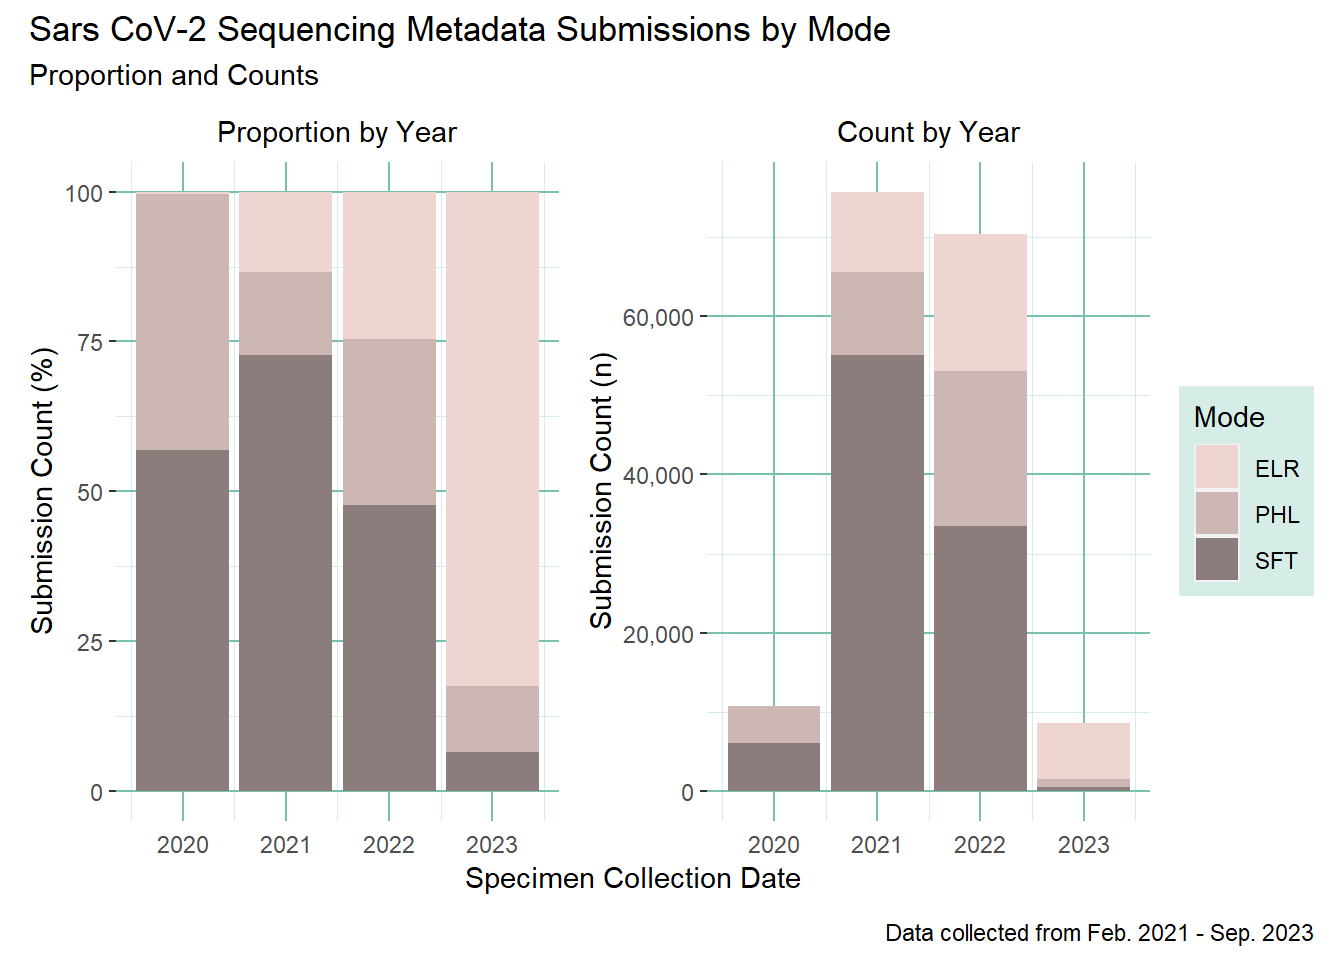
\includegraphics{index_files/figure-latex/notebooks-pipeline_counts-fig-countprop-output-1.png}

}

\caption{\label{fig-countprop}Count and proportion of sequencing
metadata submissions by mode}

\end{figure}%

\textsubscript{Source:
\href{https://NW-PaGe.github.io/sequencing_integration_pipeline1.0/notebooks/pipeline_counts-preview.html\#cell-fig-countprop}{Pipeline
Counts}}

96\% of those sequences were successfully matched to a case in WDRS,
while 3\% had no match. Less than 1\% of the records had quality issues
that could not be resolved and are still archived in our for review
process. See Table~\ref{tbl-counts} for more details.

\begin{longtable}[]{@{}ll@{}}

\caption{\label{tbl-counts}Count of sequences matching to WDRS cases}

\tabularnewline

\toprule\noalign{}
\multicolumn{2}{@{}l@{}}{%
Covid Sequencing Pipeline Counts} \\
Location & Count \\
\midrule\noalign{}
\endhead
\bottomrule\noalign{}
\endlastfoot
For Review & 220 (0.13\%) \\
Fuzzy Review & 569 (0.33\%) \\
Keep NA & 5,710 (3.32\%) \\
WDRS & 165,551 (96.22\%) \\
Total & 172,050 (-) \\

\end{longtable}

\textsubscript{Source:
\href{https://NW-PaGe.github.io/sequencing_integration_pipeline1.0/notebooks/pipeline_counts-preview.html\#cell-tbl-counts}{Pipeline
Counts}}

When stratifying by lab/submitter in Table~\ref{tbl-labcount}, we can
see that most of the sequences were submitted by 4 labs. Over 40\% of
the sequences were submitted by University of Washington Virology Lab,
followed by our own PHL with 19\%, Labcorp with 15\% and Northwest
Genomics with 11\%.

\begin{longtable}[]{@{}
  >{\raggedright\arraybackslash}p{(\columnwidth - 4\tabcolsep) * \real{0.3333}}
  >{\raggedright\arraybackslash}p{(\columnwidth - 4\tabcolsep) * \real{0.3333}}
  >{\raggedright\arraybackslash}p{(\columnwidth - 4\tabcolsep) * \real{0.3333}}@{}}

\caption{\label{tbl-labcount}Count of sequences by lab and status during
the sequencing pipeline 1.0 phase}

\tabularnewline

\toprule\noalign{}
\multicolumn{3}{@{}>{\raggedright\arraybackslash}p{(\columnwidth - 4\tabcolsep) * \real{1.0000} + 4\tabcolsep}@{}}{%
Number of Sequences by Lab} \\
\multicolumn{3}{@{}>{\raggedright\arraybackslash}p{(\columnwidth - 4\tabcolsep) * \real{1.0000} + 4\tabcolsep}@{}} \\
PHL & 32,845 & {19.8\%} \\
Labcorp & 26,597 & {16.1\%} \\
NW Genomics & 18,532 & {11.2\%} \\
Quest & 4,121 & {2.5\%} \\
Altius & 3,696 & {2.2\%} \\
Fulgent Genetics & 2,859 & {1.7\%} \\
PHL/Bedford & 2,857 & {1.7\%} \\
SCAN/Bedford & 1,004 & {0.6\%} \\
Aegis & 943 & {0.6\%} \\
Curative Labs & 649 & {0.4\%} \\
KP WA Research Inst & 281 & {0.2\%} \\
USAFSAM & 275 & {0.2\%} \\
CDC & 211 & {0.1\%} \\
Providence Swedish & 173 & {0.1\%} \\
Helix & 151 & {0.1\%} \\
Lauring Lab & 118 & {0.1\%} \\
Atlas Genomics & 89 & {0.1\%} \\
Boise VA & 67 & {0\%} \\
OHSU & 61 & {0\%} \\
SFS/Bedford & 53 & {0\%} \\
IDBOL & 40 & {0\%} \\
Gravity Diagnostics & 36 & {0\%} \\
ASU & 33 & {0\%} \\
NA & 18 & {0\%} \\
OSPHL & 15 & {0\%} \\
USAMRIID & 9 & {0\%} \\
Infinity Biologix & 7 & {0\%} \\
Grubaugh Lab & 2 & {0\%} \\
Montana Public Health Lab & 2 & {0\%} \\
Flow Diagnostics & 1 & {0\%} \\
Grittman Medical Center & 1 & {0\%} \\
NW GENOMICS & 1 & {0\%} \\
Naval Health Research Center & 1 & {0\%} \\
Providence\_Swedish & 1 & {0\%} \\
SCAB/Bedford & 1 & {0\%} \\
SFS/ Bedford & 1 & {0\%} \\
The Jackson Laboratory & 1 & {0\%} \\

\end{longtable}

\textsubscript{Source:
\href{https://NW-PaGe.github.io/sequencing_integration_pipeline1.0/notebooks/pipeline_counts-preview.html\#cell-tbl-labcount}{Pipeline
Counts}}

\href{notebooks/pipeline_counts.qmd\#tbl-labcount}{source notebook}.

\phantomsection\label{refs}
\begin{CSLReferences}{1}{0}
\bibitem[\citeproctext]{ref-olteanSentinelSurveillanceSystem}
Oltean, Hanna N., Krisandra J. Allen, Lauren Frisbie, Stephanie M. Lunn,
Laura Marcela Torres, Lillian Manahan, Ian Painter, et al. n.d.
{``Sentinel {Surveillance System Implementation} and {Evaluation} for
{SARS-CoV-2 Genomic Data}, {Washington}, {USA}, 2020--2021 - {Volume}
29, {Number} 2---{February} 2023 - {Emerging Infectious Diseases}
Journal - {CDC}.''} Accessed March 18, 2024.
\url{https://doi.org/10.3201/eid2902.221482}.

\bibitem[\citeproctext]{ref-olteanChangingGenomicEpidemiology2024}
Oltean, Hanna N., Allison Black, Stephanie M. Lunn, Nailah Smith,
Allison Templeton, Elyse Bevers, Lynae Kibiger, et al. 2024. {``Changing
Genomic Epidemiology of {COVID-19} in Long-Term Care Facilities During
the 2020--2022 Pandemic, {Washington State}.''} \emph{BMC Public Health}
24 (January): 182. \url{https://doi.org/10.1186/s12889-023-17461-2}.

\bibitem[\citeproctext]{ref-wagnerPositiveSelectionUnderlies2023}
Wagner, Cassia, Kathryn E. Kistler, Garrett A. Perchetti, Noah Baker,
Lauren A. Frisbie, Laura Marcela Torres, Frank Aragona, et al. 2023.
{``Positive Selection Underlies Repeated Knockout of {ORF8} in
{SARS-CoV-2} Evolution.''} September 23, 2023.
\url{https://doi.org/10.1101/2023.09.21.23295927}.

\end{CSLReferences}



\end{document}
